\documentclass{pracamgr}

\usepackage{polski}
\usepackage[utf8]{inputenc}
\usepackage[pdftex]{graphicx}

\usepackage{subfig} % Subfigures
\usepackage{color}
\usepackage{ntheorem} % Definitions
\usepackage{sidecap} % Side captions to figures
\usepackage{multicol}
\usepackage{listings}
\usepackage{rotating} % Sideway figures
\usepackage{array} % Same formatting for column tables
\usepackage{multirow} % Row and columns spans
\usepackage[obeyspaces, spaces]{url} %Proper line breaking for typewriter-style texts
\usepackage{caption} %Legends with \caption*
\usepackage{amsfonts}

\author{Maciej Pazurkiewicz}
\nralbumu{248267}

\title{Modelowanie sygnalizacji świetlnej}

\tytulang{Modelling of a~traffic lights system}
\kierunek{Informatyka}

\opiekun{dra hab. Sławomira Lasoty\\
  Instytut Informatyki
  }
% miesiąc i~rok:
\date{Wrzesień 2011}

%Podać dziedzinę wg klasyfikacji Socrates-Erasmus:
\dziedzina{
11.3 Informatyka\\
}

%Klasyfikacja tematyczna według AMS (matematyka) lub ACM (informatyka)
\klasyfikacja{D. Software\\
  D.2. Software engineering\\
  D.2.4. Software/Program verification}

% Słowa kluczowe:
\keywords{sygnalizacja świetlna, system czasu rzeczywistego,
  modelowanie formalne, automaty czasowe, Uppaal}

%--------------------------------------------------------------------------
% My macros
%--------------------------------------------------------------------------
\newcommand{\todo}[1]{\textcolor{red}{#1}}
\newcommand{\todocite}{\todo{[source]}}
\newcommand{\comments}[1]{}

\newcommand{\ang}[1]{(ang.~\emph{#1})}
\newcommand{\imgr}[1]{rys.~\ref{#1}}
\newcommand{\upp}{\textsc{Uppaal}}
\newcommand{\rarr}{$\rightarrow$}

\newcommand{\ttt}[1]{\url{#1}}
\newcommand{\tttform}[1]{
  \begin{center}
    \ttt{#1}
  \end{center}
}

%Math mode
\newcommand{\pair}[2]{\langle #1, #2 \rangle}
\newcommand{\floor}[1]{\lfloor #1 \rfloor}
\newcommand{\br}[1]{\{ #1 \}}

\theoremstyle{plain}
\theoremsymbol{\ensuremath{\clubsuit}}
\theoremseparator{.}
\theoremprework{\medskip\begin{samepage}}
\theorempostwork{\medskip\end{samepage}}
\newtheorem{definition}{Definicja}

%Listings
\lstdefinelanguage{Signals} {}

\lstset{
  basicstyle=\tt, extendedchars = true,
  keywordstyle=\underbar,
  emphstyle=\bf,
  %columns=fullflexible,
  xleftmargin=1cm,
  captionpos=b, abovecaptionskip=12pt, belowcaptionskip=12pt,
  delim=**[is][\ttfamily]{|}{|},
  mathescape=true,
  belowskip=.5cm,
  aboveskip=.5cm,
  language=Signals,
}
\definecolor{light-gray}{gray}{0.40}
\newcommand{\com}[1]{\upshape\color{light-gray}{#1}}

%--------------------------------------------------------------------------

\begin{document}
\maketitle

\begin{abstract}
  Praca przedstawia zastosowanie metod formalnego modelowania w
  projektowaniu sygnalizacji świetlnej. Modele zostały stworzone w
  oparciu formalizm automatów czasowych i zweryfikowane przy pomocy
  narzędzia \upp.

  W pracy zaproponowano prosty język modelowania przeznaczony
  specjalnie do specyfikacji systemów sygnalizacji
  świetlnej. Stworzone w nim opisy można automatycznie przełożyć na
  modele w języku automatów czasowych, co znacząco upraszcza proces
  modelowania przy zachowaniu płynących z niego korzyści.
\end{abstract}

\tableofcontents
\addcontentsline{toc}{chapter}{Wprowadzenie}
\chapter*{Wprowadzenie}

Weryfikacja modelowa \ang{model-checking}, wprowadzona poprzez
Clarke'a i Emersona w~1980 \cite{clarke-emerson-mc}, jest jedną z
najważniejszych metod formalnych wykorzystywanych w~dowodzeniu
poprawności programów komputerowych. W~celu jej zastosowania należy
przekształcić program w opisujący go model (np.~automat skończony),
a~pożądaną własność wyrazić jako formułę pewnej logiki
temporalnej. \emph{Model-checker} przeszukuje przestrzeń stanów
modelu, aby zweryfikować prawdziwość zadanej formuły; w~przypadku, gdy
jest ona fałszywa, dostarcza ścieżkę, stanowiącą
kontrprzykład.

Najpoważniejszym problemem związanym z weryfikacją
modelową jest tzw.~\emph{eksplozja stanów}, czyli bardzo szybki wzrost
rozmiaru przestrzeni stanów modelu przy wzroście złożoności
programu. Jednym ze sposobów poradzenia sobie z nim jest
\emph{model-checking symboliczny}, którego główną ideą jest
zastąpienie wyliczania konkretnych stanów operowaniem na symbolicznych
opisach ich zbiorów \cite{mcmillan-smc}. Technika ta znacząco redukuje
zasoby potrzebne do weryfikacji danego modelu, co pozwala na
korzystanie z \emph{model-checkingu} dla systemów przemysłowych
(m.in.~\cite{smc-industry-1}, \cite{smc-industry-2}).

Wśród systemów, dla których stosuje się weryfikację modelową, liczną
grupę stanowią systemy czasu rzeczywistego. Opracowano dla nich
specjalne języki modelowania (ich obszerny przegląd można odnaleźć w
\cite{time-in-computing}) oraz narzędzia służące do weryfikacji
(m.in.~\cite{lpw:fct95}, \cite{kronos}). Jako że, już z samej swojej
natury, systemy czasu rzeczywistego mają nieskończenie wiele stanów,
wszystkie praktycznie stosowane metody należą do symbolicznych.

\emph{Model-checking}, tak jak inne metody formalne, nie jest
pozbawiony wad. Pomimo korzystania z weryfikacji symbolicznej oraz
licznych innych technik, główną z nich pozostaje problem eksplozji
stanów, często uniemożliwiający dowodzenie poprawności dużych
systemów. Poza tym stosowanie weryfikacji modelowej jest czasochłonne
i wymaga specjalistycznej wiedzy od członków zespołu. O ile
złagodzenie kwestii eksplozji stanów wymaga w wielu przypadkach dość
zaawansowanych metod, o tyle pozostałe z wymienionych problemów można
przynajmniej częściowo rozwiązać, udoskonalając i uzupełniając
dostępne narzędzia. Propozycją takiego podejścia jest przedstawiony w
pracy język modelowania sygnalizacji świetlnej.

Sygnalizacja świetlna należy do systemów czasu rzeczywistego, dla
których używanie metod formalnych jest szczególnie wskazane. Z jednej
strony całkowita poprawność jej funkcjonowania odgrywa kluczową
rolę, jako że zależy od niej życie i zdrowie uczestników ruchu. Z
drugiej zaś -- rosnąca złożoność systemów sygnalizacji świetlnej
sprawia, że tradycyjne metody zapewnienia jakości, takie jak
testowanie, mogą okazać się niewystarczające.

W niniejszej pracy przedstawiono formalne modele systemów sygnalizacji
świetlnej stworzone w formalizmie automatów czasowych oraz język
modelowania, ułatwiający ich projektowanie.  Rozdziały \ref{c:signals}
i \ref{c:ta} zawierają informacje wstępne konieczne do zrozumienia
dalszej części pracy: pierwszy wprowadza podstawowe pojęcia związane z
opisem systemów sygnalizacji, natomiast drugi omawia teorię automatów
czasowych oraz narzędzie użyte do ich weryfikacji -- \upp.  Rozdział
\ref{c:lang} przedstawia kluczowe koncepcje związane z proponowanym
językiem modelowania sygnalizacji świetlnej. Prezentuje nie tylko jego
składnię, ale także podstawowe założenia i potencjalne korzyści
wynikające z jego stosowania. Strukturę i sposób funkcjonowania modeli
generowanych na podstawie specyfikacji w tym języku przedstawia
rozdział \ref{c:models} (sama faza przekształcania specyfikacji
w~modele została w pracy pominięta jako czysto techniczna). Rozdział
\ref{c:ver} omawia wyniki weryfikacji modeli reprezentujących
kompletne systemy sygnalizacji.

\chapter{Sygnalizacja świetlna}
\label{c:signals}

Niniejszy rozdział zawiera informacje o~systemach sygnalizacji
świetlnej niezbędne w~dalszej części pracy. Podrozdział
\ref{s:sygn-wprowadzenie} jest wprowadzeniem do tematyki sygnalizacji,
natomiast podrozdział \ref{s:sygn-szczegoly} szczegółowo omawia
funkcjonowanie sygnalizacji wzbudzanej, będącej bazowym modelem
przedstawianego języka.

Niniejszy rozdział jest oparty na raportach przygotowanych na zlecenie
amerykańskiej agencji \emph{Federal Highway Administration}
\cite{fhwa:handbook06} \cite{fhwa:timing08}.

\section{Wprowadzenie}
\label{s:sygn-wprowadzenie}

Sygnalizacją świetlną nazywamy zestaw urządzeń przekazujących
komunikaty, służące do segregacji czasowej kolidujących potoków
ruchu. Stosuje się ją najpowszechniej na skrzyżowaniach i~przejściach
dla pieszych, lecz wykorzystywana jest także w~miejscach takich jak
przejazdy kolejowe, drogi o~ruchu wahadłowym lub drogi z~pasami
o~zmiennym kierunku ruchu.

Poprawnie zaprojektowana sygnalizacja świetlna powinna zmniejszać
prawdopodobieństwo wypadków i~kolizji oraz zapewniać odpowiedni poziom
dostępności dla pieszych i~pojazdów nadjeżdżających z~kierunków
podporządkowanych. Jednocześnie powinna zachowywać jak najwyższą
wydajność skrzyżowania rozumianą jako dużą przepustowość, krótki
czas oczekiwania na sygnał zielony oraz małą liczbę
zatrzymań. Zapewnienie równowagi pomiędzy bezpieczeństwem a~wydajnością
jest kluczowym aspektem projektu sygnalizacji.

\subsection{Elementy systemu sygnalizacji świetlnej}
\label{ss:elementy} Najprostszy system sygnalizacji składa się
z~sygnalizatora oraz kontrolera, czyli układu logicznego decydującego
o~wyświetlanym sygnale. Współczesne systemy są o~wiele bardziej
skomplikowane i~mogą zawierać komponenty takie jak:
\begin{description}
  \item[czujniki] -- urządzenia, które gromadzą informacje o~aktualnym
  zapotrzebowaniu różnych uczestników ruchu na prawo przejazdu bądź
  przejścia; są to np.~pętle indukcyjne w~jezdni bądź przyciski dla
  pieszych;
  \item[kontroler lokalny] -- urządzenie zarządzające pracą grupy
  ściśle powiązanych sygnalizatorów, np.~sterujących ruchem na jednym
  skrzyżowaniu;
  \item[kontroler główny] -- urządzenie zarządzające pracą grupy
  kontrolerów lokalnych; może być odpowiedzialny np.~za synchronizację
  sygnalizacji na ciągu skrzyżowań.
\end{description}

\subsection{Tryby pracy}
\label{ss:tryby} Sygnalizacja świetlna na skrzyżowaniach pracuje
przeważnie w~trybie stałoczasowym, wzbudzanym lub kombinacji obydwu.

\paragraph{Sygnalizacja stałoczasowa} W~systemach stałoczasowych każdy
z~potoków ruchu obsługiwany jest zgodnie z~ustalonym harmonogramem,
w~którym określona jest długość każdego z~sygnałów. Akomodacja może
polegać co najwyżej na zmianie harmonogramu np. w~zależności od pory dnia.

\paragraph{Sygnalizacja wzbudzana}
W~trybie wzbudzanym kontroler korzysta z~informacji dostarczanych
przez czujniki, dzięki czemu może dostosować parametry pracy
sygnalizacji do bieżących warunków ruchu. W~zależności od tego czy
czujniki są zainstalowane dla wszystkich potoków czy tylko dla
niektórych, mówimy o~sygnalizacji \emph{w pełni wzbudzanej}
\ang{fully-actuated} lub \emph{częściowo wzbudzanej}
\ang{semi-actuated}.

W~systemach w~pełni wzbudzanych sygnalizacja dla każdego z~uczestników
ruchu uzależniona jest od danych dostarczonych przez czujnik.
W~szczególności oznacza to, że w~danym cyklu sygnał zielony otrzymują
tylko te fazy, na które jest zapotrzebowanie. Także czas trwania
poszczególnych sygnałów może być funkcją danych z~czujnika.

W~systemach częściowo wzbudzanych detekcja ruchu dotyczy tylko
niektórych potoków ruchu, np.~pieszych bądź pojazdów nadjeżdżających
z~drogi podrzędnej. Prawo przejazdu jest domyślnie przyznawane
kierunkowi głównemu; pozostałe zaś mogą je otrzymać w~wyniku
zapotrzebowania zgłoszonego przez czujnik.

\section{Sygnalizacja wzbudzana}
\label{s:sygn-szczegoly}

Niniejszy podrozdział zawiera szczegółową charakterystykę
funkcjonowania sygnalizacji wzbudzanej. Najpierw definiowane są
podstawowe pojęcia potrzebne do jego precyzyjnej specyfikacji,
następnie zaś przedstawiony jest hierarchiczny opis systemu: od
omówienia pracy pojedynczego sygnalizatora po omówienie pracy całości
sygnalizacji na skrzyżowaniu.

\subsection{Podstawowe pojęcia}
\label{ss:pojecia}

Poniżej znajdują się pojęcia, których zdefiniowanie pozwoli na
uporządkowanie i~zhierarchizowanie opisu systemu sygnalizacji
świetlnej.
\begin{description}
  \item[interwał] -- odcinek czasu, w~którym wskazanie danego
  sygnalizatora nie zmienia się; w~zależności od tego wskazania mówimy
  o~\emph{interwale zielonym}, \emph{interwale żółtym} itp.;
  \item[potok ruchu] -- pojazdy bądź piesi, których ruch kontrolowany
  jest przez jeden sygnalizator\footnote{Zauważmy, że pojazdy jadące
    przez skrzyżowanie prosto oraz skręcające mogą stanowić jeden,
    dwa, a~nawet trzy oddzielne potoki w~zależności od architektury
    skrzyżowania oraz samego systemu sygnalizacji.};
  \item[faza] -- grupa potoków ruchu, którym sygnalizacja zezwala na
  jednoczesne korzystanie ze skrzyżowania;
  \item[cykl] -- ustalony ciąg faz.
\end{description}

Sygnalizator dla pojazdów wyświetla jeden z~następujących sygnałów:
czerwony, czerwono-żółty, zielony lub żółty. W~sygnalizacji dla
pieszych opuszcza się sygnał czerwono-żółty, a~żółty zastępuje się
migającym zielonym. Opis systemu sprowadza się do pokazania sposobu
wyznaczania długości interwałów odpowiadających tym sygnałom. Należy
tu uczynić dodatkową uwagę dotyczącą interwału czerwonego. Choć w~zasadzie jego
długość dla danego sygnalizatora wyznaczana jest przez długość cyklu
pracy pozostałych, to, w~celu zapewnienia bezpieczeństwa ruchu, dla
każdego potoku wyznacza się minimalny odcinek czasu pomiędzy końcem
jego aktywności a początkiem aktywności kolidującego potoku. W tym
czasie wszystkie sygnalizatory nadają sygnał czerwony. Okres ten
nazywa się go okresem oczyszczenia \ang{clearance time, all-red time}
i~wyróżnia jako dodatkowy interwał.

Sygnały czerwono-żółty, żółty, migający zielony oraz
czerwony-czyszczący nazywamy \emph{przejściowymi}. Potoki, których
sygnalizatory wyświetlają sygnał zielony lub jeden z~przejściowych,
nazywamy \emph{aktywnymi}, pozostałe zaś
\emph{nieaktywnymi}. Analogicznie, fazę, której przynajmniej jeden
potok jest aktywny nazywamy aktywną. W~danym momencie aktywna może być
co najwyżej jedna faza.

\subsection{Detekcja ruchu}
\label{ss:detekcja} Mając na celu opis systemów wzbudzanych,
rozszerzamy zestaw definicji z~\ref{ss:pojecia} o~następujące
pojęcia:
\begin{description}
  \item[zgłoszenie] -- informacja o~zapotrzebowaniu na uruchomienie
  bądź przedłużenie sygnału zielonego przekazywana odpowiedniemu
  kontrolerowi przez czujnik,
  \item[zgłoszenie przeciwne] -- zgłoszenie pochodzące od nieaktywnego
  potoku.
\end{description}

\paragraph{Czujniki dla pojazdów} Czujniki wykrywające pojazdy mogą
pracować w~jednym z~dwóch trybów: \emph{pulsacyjnym} bądź
\emph{obecności}.  W~trybie pulsacyjnym \ang{pulse mode} czujnik jest
wzbudzany tylko w~momencie pojawienia się pojazdu w~zasięgu jego
działania.  Natomiast w~trybie obecności \ang{presence mode} czujnik
pozostaje wzbudzony przez cały czas od pojawienia się pojazdu
w~strefie detekcji aż do jej opuszczenia. Zgłoszenie ma zatem postać
sygnału punktowego w~przypadku trybu pulsacyjnego oraz ciągłego dla
trybu obecności.

W modelach sygnalizacji przedstawionych w pracy używane są wyłącznie
czujniki pracujące w trybie pulsacyjnym.

\paragraph{Czujniki dla pieszych} Urządzeniem najczęściej stosowanym w
roli czujnika dla pieszych jest przycisk. Pieszy naciskając go powoduje
przekazanie zgłoszenia odpowiedniemu kontrolerowi. Po zakończeniu
obsługi potoku dla pieszych kontroler przesyła informację zwrotną do
czujnika, który jest wtedy resetowany i~staje się gotowy na ponowne
uruchomienie.

\subsection{Opis funkcjonowania sygnalizacji na poziomie pojedynczego
potoku}
\label{ss:schemat}

\paragraph{Założenia} Bazowy schemat działania sygnalizacji wzbudzanej
oparty jest na następujących założeniach:
\begin{enumerate}
  \item sygnał zielony jest przyznawany tylko wtedy, gdy wcześniej
  wykryto oczekujące nań pojazdy;
  \item długość sygnału zielonego jest zależna od natężenia ruchu
  w~danym potoku;
  \item długość oczekiwania na sygnał zielony jest ograniczona z~góry.
\end{enumerate}

\paragraph{Schemat działania} W~celu realizacji powyższych założeń,
interwał zielony dzielimy na dwie części: \emph{początkową} oraz
\emph{rozszerzalną}. Długość części początkowej jest stała i~określana
przez parametr \emph{minimalny zielony}. Powinien on wynosić co
najmniej tyle, aby pozwalać na bezpieczne opuszczenie skrzyżowania
wszystkim pojazdom znajdującym się między czujnikiem a~linią
zatrzymania.

Długość części rozszerzalnej zależy od natężenia ruchu. W~momencie
otrzymania zgłoszenia sygnał zielony przedłużany jest o~tyle, aby
przejeżdżający pojazd mógł bezpiecznie opuścić skrzyżowanie. O
długości tego odcinka czasu decyduje parametr nazywany
\emph{wydłużeniem}). Gdy kontroler nie otrzyma kolejnego
zgłoszenia tj. wykryta zostanie luka pomiędzy nadjeżdżającymi
pojazdami, sygnał zielony zostaje przerwany (patrz
\imgr{img:gap-out}).

\begin{figure}[h] \centering
  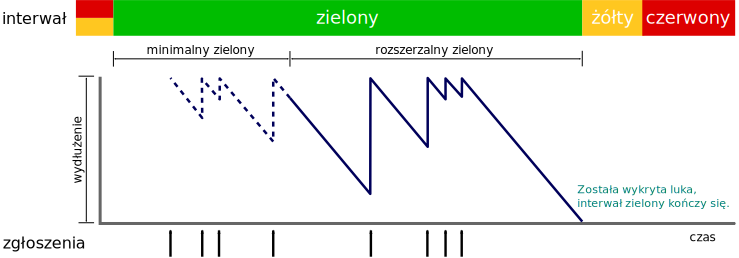
\includegraphics[width=0.7\textwidth]{img/signals-gap-out}
  \caption{Zakończenie sygnału zielonego przez wykrycie luki.}
\label{img:gap-out}
\end{figure}

Duże natężenie ruchu w~danym potoku mogłoby powodować brak luk między
pojazdami i~-- co za tym idzie~-- opóźnienia w~obsłudze
pozostałych potoków. Aby ograniczyć z~góry długość oczekiwania, określa
się maksymalny czas, w~którym potok może otrzymywać sygnał zielony
w~obecności zgłoszenia przeciwnego (patrz \imgr{img:max-out}). Należy
podkreślić, że w~razie braku zgłoszenia przeciwnego sygnał zielony
będzie nadawany tak długo aż nie nastąpi wykrycie luki.
\begin{figure}[h] \centering
  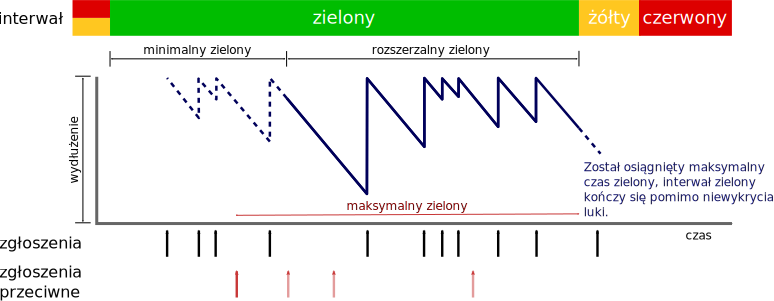
\includegraphics[width=0.7\textwidth]{img/signals-max-out}
  \caption{Zakończenie sygnału zielonego przez wykorzystanie
maksymalnego czasu.}
\label{img:max-out}
\end{figure}

\paragraph{Potoki pieszych} Tak jak w~przypadku pojazdów potok pieszy
otrzymuje sygnał zielony tylko w~wyniku zgłoszonego
zapotrzebowania. Jednak jako, że ilościowa ocena poziomu
zapotrzebowania w~przypadku ruchu pieszych jest trudna technicznie,
przyjmujemy stałą długość interwału zielonego.

\subsection{Opis funkcjonowania sygnalizacji na poziomie pojedynczej
fazy}

Podstawowym elementem opisu fazy jest stwierdzenie, które potoki
wchodzą w~jej skład. Faza może obejmować:
\begin{samepage}
\begin{itemize}
  \item jeden lub więcej potoków pojazdów,
  \item jeden lub więcej potoków pieszych,
  \item kombinację pewnej liczby potoków pojazdów i~pieszych.
\end{itemize}
\end{samepage}
\begin{figure}[h] \centering \subfloat[Faza wyłącznie dla pojazdów]{
    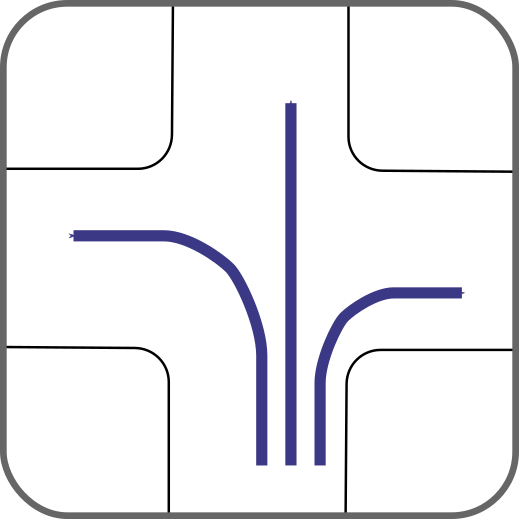
\includegraphics[width=0.27\textwidth]{img/signals-phase-example-1}
} \hfill \subfloat[Faza dla pojazdów oraz pieszych]{
    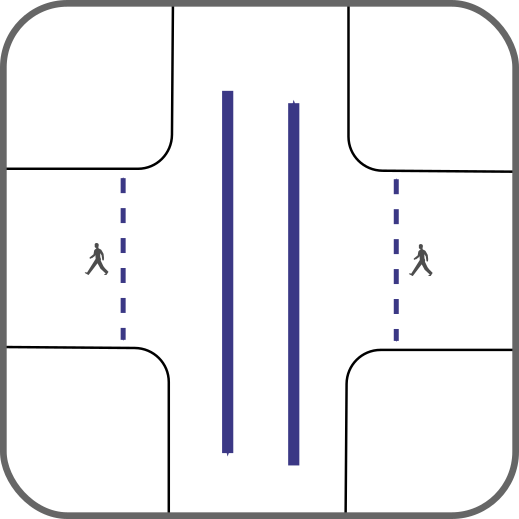
\includegraphics[width=0.27\textwidth]{img/signals-phase-example-2}
} \hfill \subfloat[Faza wyłącznie dla pieszych \ang{pedestrian
scramble, X~crossing}]{
    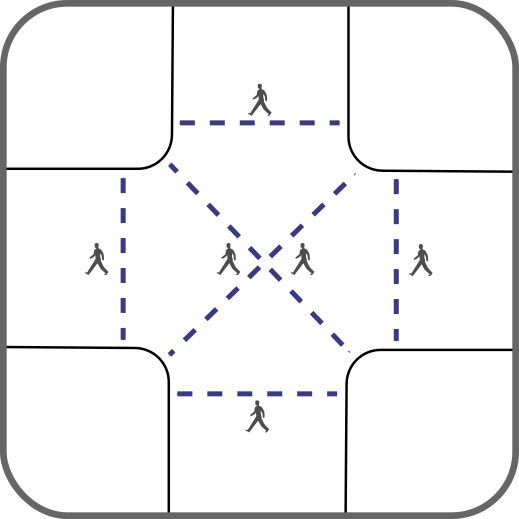
\includegraphics[width=0.27\textwidth]{img/signals-phase-example-3}
}
  \caption{Przykładowe fazy.}
\end{figure}

Zauważmy, że choć już w~opisie na poziomie potoku zaszła konieczność
zdefiniowania czasu maksymalnego, to powinien być on uważany za
właściwość fazy. Ustalenie różnych czasów maksymalnych dla różnych
potoków obniżałoby jedynie wydajność skrzyżowania w~nieuzasadniony
sposób.

Dla faz jednopotokowych nie ma potrzeby podejmowania na tym etapie
żadnych dodatkowych decyzji projektowych, gdyż opis funkcjonowania
takiej fazy jest tożsamy z~opisem funkcjonowania jej jedynego
potoku. Charakterystyka faz składających się z~wielu potoków może być
bardziej złożona, jako że dopuszczają one większą liczbę możliwych
scenariuszy. Dotyczą one sytuacji, w~których okres aktywności jednego
z~potoków mógłby być różny od okresu aktywności fazy.

\paragraph{Zgłoszenia późne} Zgłoszeniem późnym \ang{late call} nazywamy zgłoszenie od
nieaktywnego potoku, które otrzymano już po tym, gdy faza, do której
należy, stała się aktywna. Istnieją dwa sposoby obsługi takiego
zgłoszenia. Po pierwsze można uznać, że zostanie ono obsłużone dopiero
w~następnym cyklu sygnalizacji (w takim wypadku traktowane jest tak
samo jak zgłoszenia przeciwne). Drugą możliwością jest obsługiwanie
takiego zgłoszenia w~bieżącym cyklu, o~ile nie spowoduje to
przekroczenia maksymalnej długości sygnału zielonego.
\begin{figure}
  \centering
  \subfloat[Opcja podtrzymania dla potoku~1 wyłączona.]{
    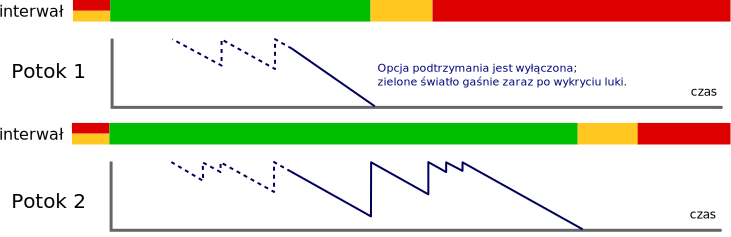
\includegraphics[width=0.8\textwidth]{img/signals-hold-1}
    \label{img:signals-hold-off}
  }\\\vspace{0.5cm}
  \subfloat[Opcja podtrzymania dla potoku~1 włączona.]{
    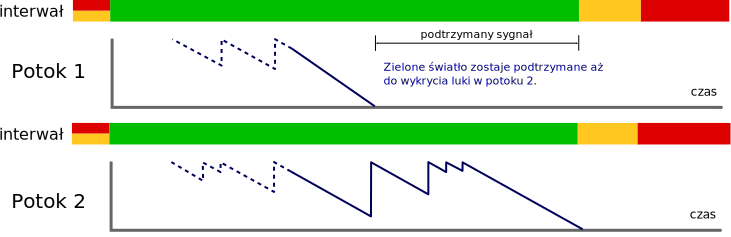
\includegraphics[width=0.8\textwidth]{img/signals-hold-2}
    \label{img:signals-hold-on}
  }
  \caption{Opcja podtrzymania sygnału dla fazy dwupotokowej.}
\end{figure}
\paragraph{Podtrzymanie} Innym elementem projektu wielopotokowej fazy
jest ustalenie zachowania się systemu w~przypadku, gdy w~jednym
z~aktywnych potoków wykryta została luka, w~innym zaś mamy do
czynienia z~ciągłym zapotrzebowaniem. Możemy nie podejmować żadnego
specjalnego działania tj. wyłączyć sygnał zielony dla potoku, w~którym
czujnik wykrył lukę (\imgr{img:signals-hold-off}). Można w~takim
przypadku zastosować także procedurę \emph{podtrzymania sygnału}
\ang{hold}. Polega ona na wydłużeniu sygnału zielonego aż do końca
aktywności fazy, tj. momentu, w~którym zakończą się sygnały zielone
dla wszystkich pozostałych potoków (\imgr{img:signals-hold-on}).

\subsection{Opis funkcjonowania sygnalizacji na poziomie cyklu}
Opis cyklu zawiera przede wszystkim informację o~kolejności
wchodzących w~jego skład faz.
\begin{figure} \centering
  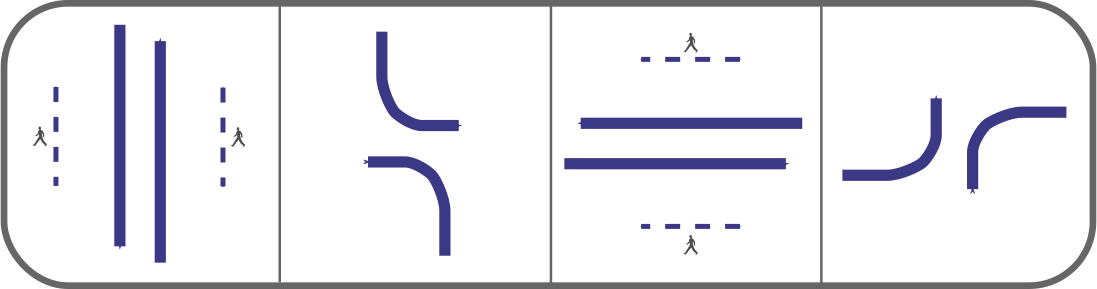
\includegraphics[width=0.7\textwidth]{img/signals-cycle-example}
  \caption{Przykładowy cykl.}
\end{figure}
Jedyną dodatkową decyzją pozostającą do podjęcia na tym etapie jest
zachowanie się sygnalizacji w~przypadku braku zgłoszeń tj.
w~\emph{stanie spoczynku} \ang{rest}. Stosowane są dwa rozwiązania. Po
pierwsze wszystkie sygnalizatory mogą wyświetlać sygnał czerwony
\ang{rest in red}. Po drugie można wybrać fazę domyślną, która będzie
aktywna w~przypadku braku jakiegokolwiek zapotrzebowania.

\subsection{Podsumowanie}
\label{ss:signals:actuated:summary}
W~rozdziale zaprezentowany został kompozycjonalny sposób opisu
systemów sygnalizacji wzbudzanej. Na początku zdefiniowano zachowanie
się sygnalizacji dla pojedynczego potoku, następnie potoki zostały
złożone w~fazy, a~fazy -- w~cykl. Na każdym etapie dokładamy
informacje specyfikujące sposób owego złożenia.

Poniższe zestawienie podsumowuje parametry zawarte w~poszczególnych
warstwach opisu.
\begin{enumerate}
  \item \textbf{Potok ruchu:}
  \begin{itemize}
    \item typ potoku: dla pojazdów / dla pieszych,
    \item tryb pracy i~rozmieszczenie czujników,
    \item długości interwałów przejściowych:
    \begin{itemize}
      \item czerwono-żółty,
      \item żółty,
      \item okres czyszczenia;
    \end{itemize}
    \item parametry decydujące o~długości interwału zielonego:
    \begin{itemize}
      \item minimalny zielony,
      \item wydłużenie;
    \end{itemize}
  \end{itemize}
  \item \textbf{Faza:}
  \begin{itemize}
    \item potoki składające się na fazę,
    \item maksymalny zielony,
    \item obsługa zgłoszeń późnych,
    \item podtrzymanie sygnału zielonego;
  \end{itemize}
  \item \textbf{Cykl:}
  \begin{itemize}
    \item fazy wchodzące w~skład cyklu i~ich kolejność,
    \item zachowanie w~stanie spoczynku.
  \end{itemize}
\end{enumerate}

\chapter{Automaty czasowe}
\label{c:ta}
Automaty czasowe są teoretycznym narzędziem umożliwiającym modelowanie
i~weryfikację systemów czasu rzeczywistego. Po zdefiniowaniu ich przez
Alura i~Dilla \cite{alur-dill} nie tylko stały się popularnym obszarem
badań teoretyków, lecz były także stosowane w~praktycznych problemach
weryfikacyjnych.

Podrozdział \ref{ta-theory} wprowadza definicję automatów czasowych
oraz zawiera najważniejsze informacje z~zakresu ich teorii;
natomiast \ref{uppaal} opisuje \upp-a -- zastosowane w~pracy narzędzie
do weryfikacji systemów modelowanych przy pomocy automatów czasowych.

\section{Automaty czasowe}
\label{ta-theory}

Formalizm automatów czasowych przedstawiony w~niniejszym
rozdziale pochodzi od  Henzingera i~in.\cite{henz-94}. Jego teoretyczna
siła wyrazu jest identyczna z~siłą wyrazu automatów w~wersji Alura
i~Dilla, natomiast jest on wygodniejszy w praktycznym modelowaniu
systemów.

Automat czasowy jest zwykłym automatem skończonym rozszerzonym
o~zestaw zmiennych rzeczywistych nazywanych zegarami. Konfiguracją
takiego automatu będziemy nazywali parę składającą się ze:
\begin{itemize}
  \item stanu odpowiedniego automatu skończonego,
  \item wartościowania zegarów.
\end{itemize}
W~konfiguracji początkowej wartości wszystkich zegarów są wyzerowane,
natomiast w~czasie działania automatu wszystkie zwiększają swoją wartość
w~tym samym tempie. Przyrost wartości zegarów modeluje upływ czasu.

Aby móc modelować systemy o~pożądanych własnościach, możemy nakładać
pewne dodatkowe warunki na tranzycje oraz stany. Każdej
tranzycji możemy przypisać wyrażenie opisujące wartościowanie zegarów,
przy którym jej wykonanie jest dozwolone. Analogiczne ograniczenia dla
stanów nazywane są \emph{niezmiennikami}. Poprawne są tylko te
konfiguracje automatu czasowego, w~których wartościowanie zegarów spełnia
niezmiennik bieżącego stanu. Jedyną dozwoloną operacją na zegarze
jest jego resetowanie, czyli ustawienie jego wartości na
zero. Przykładowy automat przedstawiono na \imgr{img:ta-simple}.

\begin{SCfigure}[4]
  \centering
  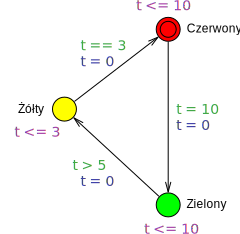
\includegraphics[width=0.3\textwidth]{img/ta-simple}
  \caption {Przykładowy automat czasowy z~jednym zegarem~$t$.
    Czcionką zieloną oznaczone są ograniczenia na krawędzie, fioletową
    niezmienniki stanów, zaś niebieską -- operacje resetowania
    zegara.\\ Automat zaczyna pracę w~stanie czerwonym, w~którym
    przebywa dokładnie przez 10 jednostek czasu. Następnie przechodzi
    do stanu zielonego (5-10 jednostek, niedeterministycznie)
i~    pomarańczowego (dokładnie 3~jednostki), po czym powraca do stanu
    początkowego.}
  \label{img:ta-simple}
\end{SCfigure}

\subsection{Formalna definicja} Przyjmijmy, że mamy skończony zbiór
$\mathcal{C}$ zmiennych rzeczywistych (zegarów) oraz skończony alfabet
$\Sigma$ (akcji).
\begin{definition}[Ograniczenie zegarowe] Ograniczeniem zegarowym
nazywamy koniunkcję formuł o~postaci $x \sim n$,
gdzie $x\in\mathcal{C}$, $n \in \mathbb{N}$, natomiast $\sim$
jest jedną spośród relacji \mbox{$=, <, \leq, >, \geq$}.
\end{definition}
Zbiór ograniczeń zegarowych nad $\mathcal{C}$ będziemy oznaczali przez
$\mathcal{B}(\mathcal{C})$\footnote{W \cite{henz-94} ograniczenia mogą
mieć także postać: $x - y \sim n$.}.

\begin{definition}[Automat czasowy] Automat czasowy jest $\mathcal{A}$
jest krotką $\langle L, l_0, E, I\rangle$, gdzie
  \begin{itemize}
    \item $L$ jest skończonym zbiorem stanów,
    \item $l_0$ jest stanem początkowym,
    \item $E \subseteq L~\times \mathcal{B}(\mathcal{C}) \times \Sigma
    \times 2^{\mathcal{C}} \times L$ jest zbiorem krawędzi,
    \item $I: L~\mapsto \mathcal{B}(\mathcal{C})$ jest funkcją
    przypisującą stanom ich niezmienniki.
  \end{itemize}
\end{definition}
Zamiast $\langle l, g, a, r, l' \rangle \in E$ będziemy pisali $l
\stackrel{g, a, r}{\longrightarrow} l'$. Zapis taki oznacza tranzycję
$a$ prowadzącą ze~stanu $l$ do stanu $l'$, którą można
wykonać przy wartościowaniu zegarów spełniającym ograniczenie $g$
i~przypisującą $0$ wszystkim zegarom z~$r$.

Tak zdefiniowany automat czasowy rozumiemy jako
system przejść, w~którym można wykonywać dwa rodzaje tranzycji:
\begin{description}
  \item[upływ czasu] polega na zwiększeniu wartości wszystkich zegarów
  o~pewną liczbę rzeczywistą; intuicyjnie, jest to przebywanie przez
  jakiś czas w~którymś ze~stanów;
  \item[wykonanie akcji] polega na przejściu do innego stanu
  zgodnie z~wybraną krawędzią; wykonanie akcji nie jest związane
  z~upływem czasu (zmiana wartościowania zegarów może wynikać jedynie
  ze zresetowania niektórych z~nich).
\end{description}
Formalnie ujmuje to poniższa definicja.
\begin{definition}[Semantyka operacyjna automatu czasowego] Semantyką
  automatu czasowego jest system przejść, którego stany są parami
  $\pair{l}{\mu} \in L \times (\mathbb{R}^+)^{\mathcal{C}}$ a~przejścia
  spełniają następujące reguły:
  \begin{itemize}
    \item $\pair{l}{\mu} \stackrel{d}{\longrightarrow} \pair{l}{\mu+d}$,
    jeśli $\mu \vdash I(l)$ oraz $(\mu+d) \vdash I(l)$ dla pewnego
    dodatniego $d \in \mathbb{R}^{+}$
    \item $\pair{l}{\mu} \stackrel{a}{\longrightarrow} \pair{l'}{\mu'}$,
    jeśli $l \stackrel{g, a, r}{\longrightarrow} l', \mu~\vdash g, \mu' =
    \mu[r \mapsto 0]$ oraz $\mu \in I(l)$ i $\mu' \in I(l')$
  \end{itemize}
\end{definition}

\subsection{Problemy weryfikacyjne}
\label{ss:ta:theory:verification}
Liczba konfiguracji tak zdefiniowanego automatu jest nieprzeliczalna, co
sprawia, że wydaje się, że nie stanowi on odpowiedniego modelu dla zadań
weryfikacyjnych. Rozwiązanie tego problemu zaproponowali już Alur
i~Dill \cite{alur-dill}, zauważając, że pewnych własności można dowodzić,
opierając się na skończonej abstrakcji automatu.

Wprowadzona przez nich abstrakcja nazywa się \emph{równoważnością
  regionów}. Opiera się na spostrzeżeniu, że dwa stany automatu są
równoważne, gdy:
\begin{samepage}
\begin{enumerate}
  \item wartości zegarów zgadzają się co do części całkowitej,
  \item zachowany jest porządek na częściach ułamkowych zegarów.
\end{enumerate}
\end{samepage}
Intuicyjnie, pierwsza własność odpowiada za sprawdzenie czy spełnione
jest dane ograniczenie zegarowe; natomiast dzięki drugiej wiadomo,
wartość którego zegara przekroczy jako pierwsza kolejną liczbę
naturalną \cite{am:decision}. Po dodatkowym utożsamieniu ze sobą
stanów, w~których wartości zegarów są większe niż odpowiednie
maksymalne stałe z~ograniczeń, zyskujemy skończoną abstrakcję dla
wartościowań zegarów (rys. \ref{img:regions}).
\begin{figure}
  \centering
  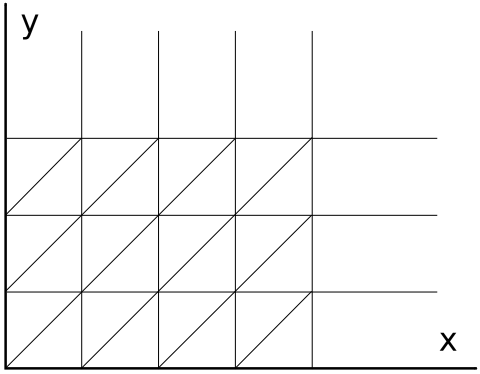
\includegraphics[width=0.4\textwidth]{img/ta-regions}
  \caption{Regiony dla automatu o~dwóch zegarach (każdy punkt
    przecięcia, odcinek, półprosta oraz ograniczony nimi fragment
    płaszczyzny reprezentują oddzielny region).}
  \label{img:regions}
\end{figure}

Relację równoważności regionów formalizuje się w następujący sposób.
Dla dowolnego $d\in\mathbb{R}$ przez $\floor{d}$ oznaczamy część
całkowitą $d$, a przez $\br{d}$ jego część ułamkową; dla każdego~$d$
mamy zatem: $d = \floor{d} + \br{d}$. Dla każdego zegara $t$ przez
$C_t$ oznaczamy największą liczbę, z którą $t$ jest porównywany w
ograniczeniach. Równoważność regionów jest relacją na zbiorze
wartościowań zegarów danego automatu.
\begin{definition}[Równoważność regionów]
  Dwa wartościowania zegarów $\mu$ i $\nu$ są równoważne, gdy
  spełniają następujące warunki:
  \begin{enumerate}
    \item Dla każdego zegara $t\in\mathcal{C}$: albo $\floor{\mu(t)} =
    \floor{\nu(t)}$, albo zarówno $\mu(t)$ jak i $\nu(t)$ przekraczają $C_t$.
    \item Dla każdej pary zegarów $t, z$ takich, że zachodzi $\mu(t)
    \leq C_t$ i $\mu(z) \leq C_z$:\\ \mbox{$\br{\mu(t)} \leq
      \br{\mu(z)} \iff \br{\nu(t)} \leq \br{\nu(z)}$}.
    \item Dla każdego zegara $t$ takiego, że zachodzi $\mu(t) \leq
    C_t$: $\br{\mu(t)}=0 \iff \br{\nu(t)}=0$.
  \end{enumerate}

\end{definition}

Dla automatu czasowego $A$ konstruuje się tzw. \emph{automat
  regionów}.

\begin{definition}[Automat regionów]
  Automatem regionów $R(A)$ dla automatu czasowego $A$ nazywamy
  automat, którego konfiguracje są parami $\pair{l}{r}$, gdzie $l$
  jest stanem automatu $A$, zaś $r$ pewnym regionem. W $R(A)$ mamy
  następujące krawędzie:
  \begin{itemize}
    \item $\pair{l}{r} \stackrel{d}{\longrightarrow} \pair{l}{r'}$ dla
    dodatniego $d\in\mathbb{R}^+$, gdy dla pewnych wartościowań
    zegarów $\mu\in r$ oraz $\mu'\in r'$ mamy w $A$ tranzycję 
    $\pair{l}{\mu} \stackrel{d}{\longrightarrow} \pair{l}{\mu'}$,
    \item $\pair{l}{r} \stackrel{a}{\longrightarrow} \pair{l'}{r'}$
    dla $a\in\Sigma$, gdy dla pewnych wartościowań
    zegarów $\mu\in r$ oraz $\mu'\in r'$ mamy w $A$ tranzycję
    $\pair{l}{\mu} \stackrel{a}{\longrightarrow} \pair{l'}{\mu'}$.
  \end{itemize}

\end{definition}

Automat regionów jest zwykłym automatem skończonym, zatem można dla
niego efektywnie rozstrzygać np.~osiągalność konfiguracji bądź
pustość języka, co przekłada się na rozstrzygalność tych problemów
dla automatów czasowych.

Chociaż równoważność regionów jest bardzo wygodnym pojęciem
w~teoretycznych badaniach własności automatów czasowych, nie stosuje się
go w~rzeczywistych problemach weryfikacyjnych. Rozmiar automatu
regionów jest bowiem wykładniczy ze względu na liczbę zegarów oraz
górne ograniczenia ich wartości.

Bardziej zgrubnej -- niemniej wystarczająco dokładnej dla
weryfikacji -- abstrakcji wartościowań zegarów dokonuje się przy pomocy
\emph{stref} \ang{zones} \cite{henz-94}.
\begin{definition}
  Strefą nazywamy maksymalny zbiór wartościowań zegarów spełniających
  koniunkcję pewnych ograniczeń zegarowych.
\end{definition}
Przykłady graficznej reprezentacji stref przedstawia rysunek
\ref{img:zones}; zauważmy, że każda strefa jest wypukłą sumą pewnej
liczby regionów.
\begin{figure}
  \centering
  \subfloat[Strefa $y \geq 1$.]{
    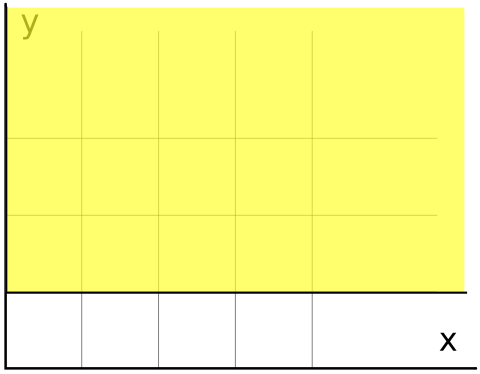
\includegraphics[width=0.35\textwidth]{img/ta-zone-1}
  }
  \hspace{1.5cm}
  \subfloat[Strefa $1 \leq x \leq 4 \land 1 \leq y \leq 3$.]{
    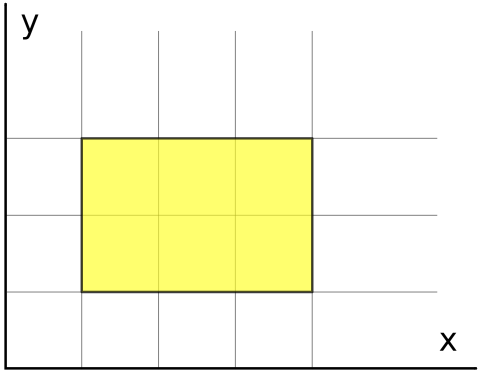
\includegraphics[width=0.35\textwidth]{img/ta-zone-2}
  }
  \caption{Przykładowe strefy.}
  \label{img:zones}
\end{figure}

Analogicznie, do automatu regionów konstruuje się automat stref.
Rysunek \ref{img:zones-automaton} przedstawia automat czasowy
i~odpowiadający mu automat stref. Zauważmy, że powiększenie stałych
z~ograniczeń nie wpłynęłoby na rozmiar automatu stref, natomiast
zdecydowanie zwielokrotniłoby rozmiar automatu regionów. Rozmiar
automatu stref zależy wyłącznie od liczby istotnie różnych
konfiguracji wyjściowego automatu czasowego.
\begin{figure}
  \centering
  \subfloat[Przykładowy automat czasowy.] {
    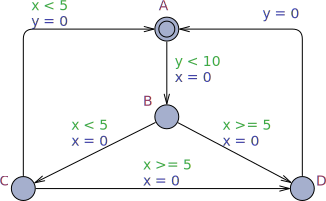
\includegraphics[width=0.35\textwidth]{img/ta-zones-example-1}
  } \hspace{1cm}
  \subfloat[Odpowiadający mu automat stref.] {
    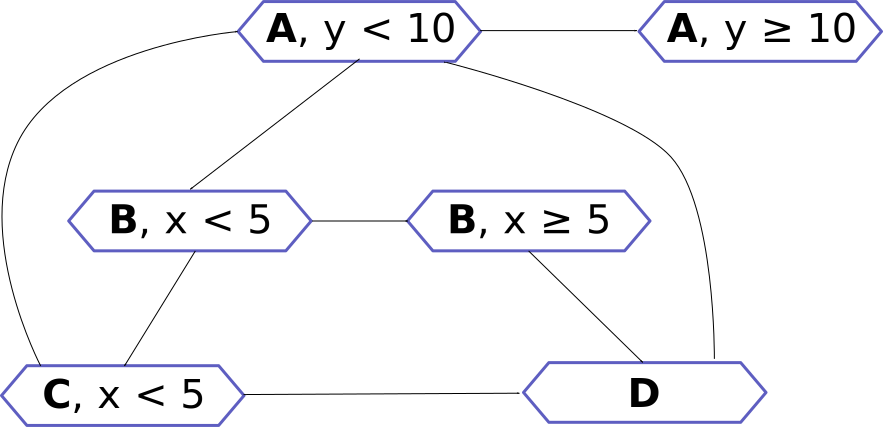
\includegraphics[width=0.35\textwidth]{img/ta-zones}
  }
  \caption{Automat stref.}
  \label{img:zones-automaton}
\end{figure}

\section{\upp}
\label{uppaal}

\upp\ jest zestawem narzędzi pozwalającym na modelowanie systemów czasu
rzeczywistego przy pomocy automatów czasowych, ich symulację, a~także
weryfikację ich własności. Rozwijają go wspólnie Uniwersytet w~Uppsali
oraz Uniwersytet w~Aalborg. Pierwsza wersja narzędzia została wydana w~roku
1995 \cite{lpw:fct95}.

\upp\ był wielokrotnie wykorzystywany w~weryfikacji rzeczywistych
systemów: od protokołów komunikacyjnych po aplikacje multimedialne
(m.in. \cite{lp:prfts97}, \cite{lpw:tacas98},
\cite{DBLP:conf/icfem/BordbarO03},
\cite{Ravn:2011:MVW:1987389.1987431}). Był jednym z~głównym narzędzi
stosowanych w~-- prowadzonym przez konsorcjum europejskich
uniwersytetów i~przedsiębiorstw -- projekcie \textsc{Ametist}, mającym
na celu rozwój efektywnych metod weryfikacji przemysłowych systemów czasu
rzeczywistego \cite{AMETISTfinal}.

\subsection{Modelowanie}
Modelowanie w~\upp-u polega nie tyle na tworzeniu jednego automatu
czasowego, lecz projektowaniu \emph{szablonów} automatów, których
instancje -- nazywane procesami -- tworzą model całego systemu. Dzięki
temu model można podzielić na logiczne części o~określonych
odpowiedzialnościach.

Model projektuje się przy pomocy prostego graficznego interfejsu
użytkownika (patrz rys.~\ref{img:uppaal-gui}). Wbudowany w~aplikację
symulator pozwala na szybkie zapoznanie się z~funkcjonowaniem modelu,
a~także ułatwia przeglądanie kontrprzykładów dostarczanych przez
weryfikator. Co ważne, symulator pokazuje nie konkretne stany systemu,
a~stany symboliczne (strefy). Przydatną funkcją jest także generacja
diagramu komunikacji procesów w~trakcie symulacji
(rys.~\ref{img:uppaal-msc}).
\begin{figure}
  \centering
  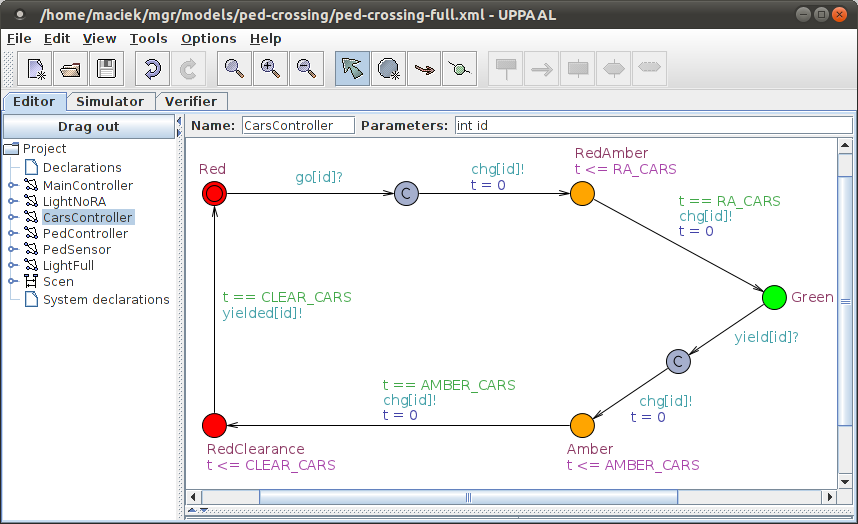
\includegraphics[width=0.9\textwidth]{img/uppaal-editor.png}
  \caption{Interfejs edytora szablonów procesów.}
  \label{img:uppaal-gui}
\end{figure}

\begin{figure}
  \centering
  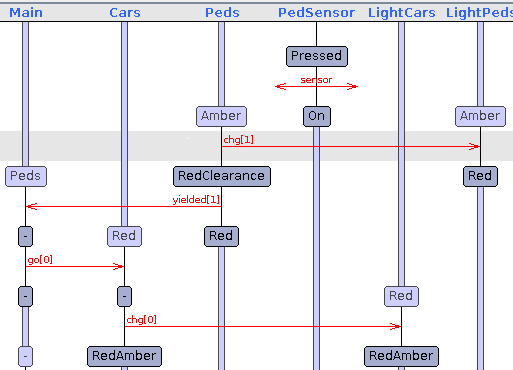
\includegraphics[width=0.8\textwidth]{img/uppaal-msc.png}
  \caption{Generowany przez symulator \upp-a diagram komunikacji
    procesów \ang{message sequence chart}.}
  \label{img:uppaal-msc}
\end{figure}

Autorzy \upp-a rozszerzyli podstawową definicję automatów czasowych
o~dodatkowe konstrukcje. Większość nie zwiększa siły
wyrazu formalizmu, a~jedynie ułatwia modelowanie bardziej złożonych
systemów.  Poniżej opisane zostaną najważniejsze rozszerzenia
(ich wyczerpujący opis wraz z~formalnie zdefiniowaną semantyką
odnaleźć można w~\cite{by-lncs04}).
\paragraph{Procesy i~ich komunikacja} Możliwość modelowania przy
pomocy sieci automatów czasowych wiąże się z~koniecznością
wprowadzenia mechanizmu komunikacji pomiędzy poszczególnymi
procesami. W~\upp-u jest ona realizowana poprzez synchronizację na
kanałach komunikacyjnych. Dwa procesy synchronizują się na kanale
komunikacyjnym \texttt{a}, gdy jeden z~nich wykonuje z~nich
akcję~\texttt{a?}, a~drugi --~\texttt{a!}. Kanał komunikacyjny może
być zadeklarowany także jako \emph{rozgłoszeniowy} \ang{broadcast}, co
pozwala na synchronizację \emph{jeden do wielu}.
\begin{SCfigure}[3]
  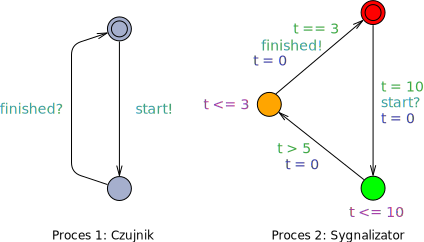
\includegraphics[width=0.6\textwidth]{img/ta-communication}
  \caption[Synchronizujące się ze sobą automaty czasowe.]
  {Synchronizujące się ze sobą automaty czasowe. System składa się
    z~dwóch procesów: czujnika i~sygnalizatora. Proces sygnalizatora
    przypomina ten z~\imgr{img:ta-simple}; w~tym wypadku jednak czas
    przebywania w~stanie czerwonym nie jest stały, lecz wyznaczany
    przez proces czujnika. Czujnik wysyła polecenie początku pracy
    \texttt{start!}, a~następnie czeka na informację o~jej zakończeniu
    na kanale \texttt{finished}.}
\end{SCfigure}

\paragraph{Zmienne całkowitoliczbowe} Obok zmiennych zegarowych
użytkownik może deklarować także zmienne całkowitoliczbowe oraz
tablice. Wyrażeń na nich można używać w~ograniczeniach na krawędziach
oraz niezmiennikach stanów. Przypisania na zmienne wykonywane są
w~trakcie przejścia, analogicznie do resetowania zegarów.

\paragraph{Stany pilne oraz uprzywilejowane} Wprowadzono możliwość
dodatkowego oznaczenia stanów automatu jako \emph{pilne}
\ang{urgent} bądź \emph{uprzywilejowane} \ang{committed}.

Jeśli automat jest w~stanie pilnym, nie może wykonać tranzycji,
polegającej na upływie czasu. Jest to równoważne zadeklarowaniu
dodatkowego zegara $t$, który będzie resetowany na wszystkich
krawędziach wchodzących do danego stanu oraz nadaniu mu
niezmiennika $t \leq 0$ (\imgr{img:uppaal-urgent}). Jako pilne mogą
być oznaczone także kanały komunikacyjne; procesy muszą się
zsynchronizować na takim kanale tak szybko jak będzie to możliwe.

\begin{figure}[h]
  \centering
  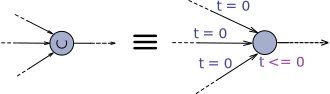
\includegraphics[width=.5\textwidth]{img/uppaal-urgent}
  \caption{Stan pilny i~równoważny mu stan z~dodatkowym
    zegarem.}
  \label{img:uppaal-urgent}
\end{figure}

Jeszcze silniejszą własność mają stany uprzywilejowane. Są to stany
pilne, z~których przejście należy wykonać tak szybko jak to
możliwe. Jeśli któryś z~procesów jest w~stanie uprzywilejowanym,
system nie może wykonać przejścia ze stanu nieuprzywilejowanego.
Stany uprzywilejowane są bardzo przydatne np.~w~modelowaniu atomowych
ciągów komunikacji pomiędzy wieloma procesami.

\subsection{Weryfikacja}

Weryfikator \upp-a pozwala na dowodzenie własności opisywanych przez
podzbiór języka TCTL \cite{acd:mc}. Poprawne są wszystkie formuły
następujących postaci \cite{by-lncs04}:
\begin{itemize}
  \item \texttt{A[] $\varphi$} -- ,,zawsze $\varphi$'' (bezpieczeństwo),
  \item \texttt{E<> $\varphi$} -- ,,być może kiedyś $\varphi$''
  (osiągalność),
  \item \texttt{A<> $\varphi$} -- ,,zawsze kiedyś $\varphi$'',
  \item \texttt{E[] $\varphi$} -- ,,być może zawsze $\varphi$''
  \item \texttt{$\varphi$ --> $\psi$}\footnote{W czystym TCTL własność
    ta zostałaby zapisana następująco: \texttt{A[]
      ($\varphi\rightarrow$ A<> $\psi)$}} -- ,,$\varphi$ zawsze
  prowadzi do $\psi$'' (żywotność),
\end{itemize}
gdzie $\varphi$ i~$\psi$ są własnościami pojedynczej konfiguracji
tj. predykatami dotyczącymi stanów oraz zmiennych liczbowych
i~zegarów. Dodatkowo dostępny jest predykat \texttt{deadlock} prawdziwy
w~stanach, w~których nastąpiło zakleszczenie tj. nie można wykonać
żadnego dozwolonego przejścia. Formułując własności konfiguracji,
mozna korzystać ze standardowych operatorów logicznych, np.:

\begin{samepage}
\begin{itemize}
  \item \url{P1.A and P1.t <= 10} -- automat \url{P1} jest w stanie
  \url{A}, zaś jego zegar \url{t} ma wartość mniejszą bądź równą 10;
  \item \url{P1.A imply P2.B} -- jeśli automat \url{P1} jest w stanie
  \url{A}, to automat \url{P2} jest w stanie \url{B}.
\end{itemize}
\end{samepage}

Semantykę powyższych formuł określamy, rozwijając kolejne
przejścia w~potencjalnie nieskończone drzewo. Litery \texttt{A}
i~\texttt{E} w~formułach wprowadzają kwantyfikację po ścieżkach tego drzewa:
\texttt{A} oznacza, że dana własność ma być spełniona dla wszystkich
ścieżek, zaś \texttt{E} -- dla co najmniej jednej. Symbole
\texttt{[]} oraz \texttt{<>} kwantyfikują stany na pojedynczej
ścieżce: \texttt{[]} mówi, że własność ma być spełniona dla wszystkich
stanach na ścieżce, zaś \texttt{<>} -- w~co najmniej jednym.

\begin{figure}
  \centering
  \subfloat[{\texttt{A[] $\varphi$}}]{
    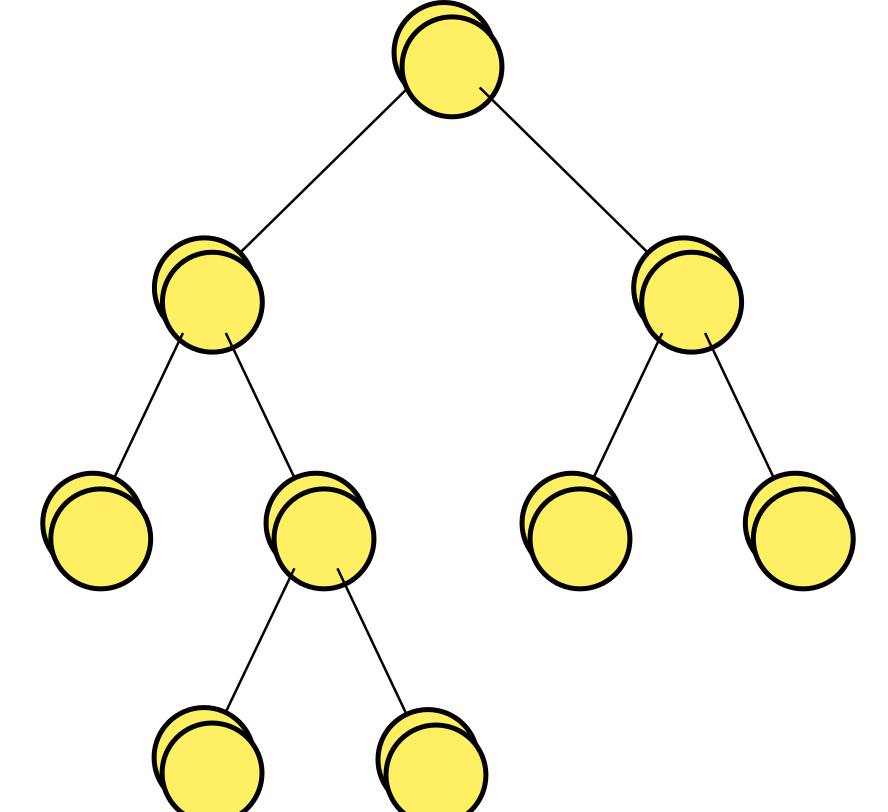
\includegraphics[width=0.3\textwidth]{img/uppaal-tctl-1}
  }
  \subfloat[\texttt{A<> $\varphi$}]{
    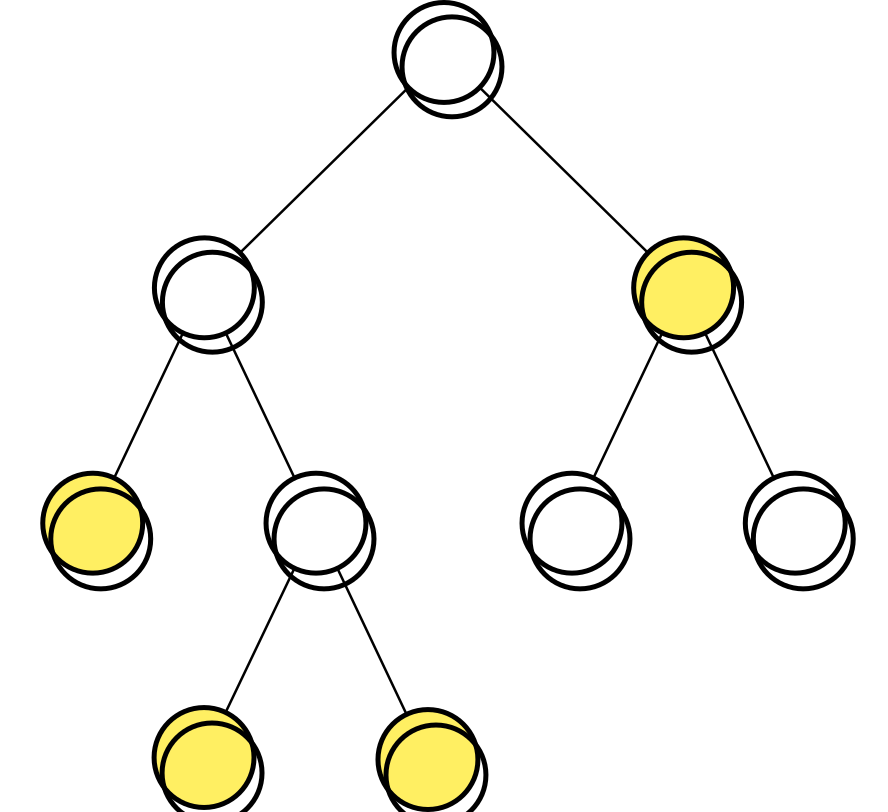
\includegraphics[width=0.3\textwidth]{img/uppaal-tctl-2}
  }\\
  \subfloat[\texttt{E[] $\varphi$}]{
    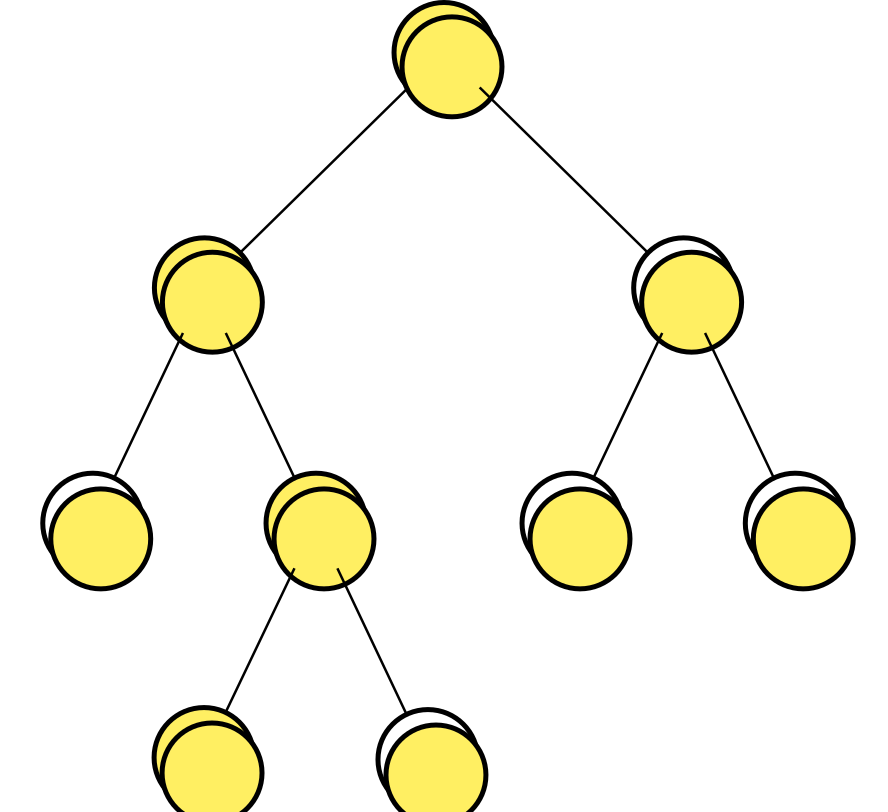
\includegraphics[width=0.3\textwidth]{img/uppaal-tctl-3}
  }
  \subfloat[\texttt{E<> $\varphi$}]{
    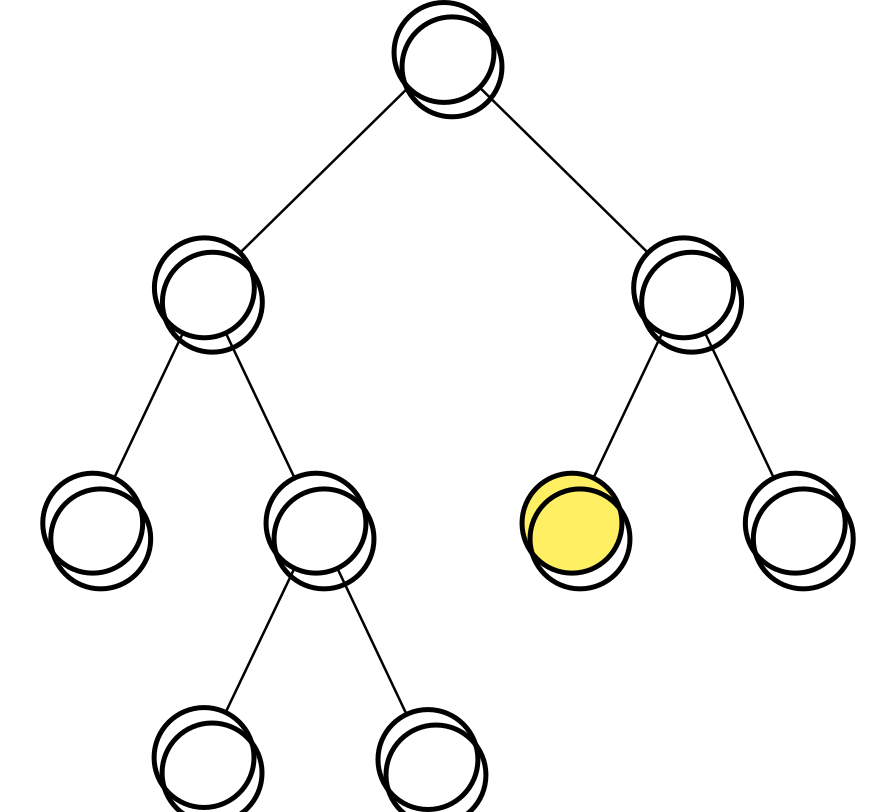
\includegraphics[width=0.3\textwidth]{img/uppaal-tctl-4}
  }
  \subfloat[\texttt{$\varphi$ --> $\psi$}]{
    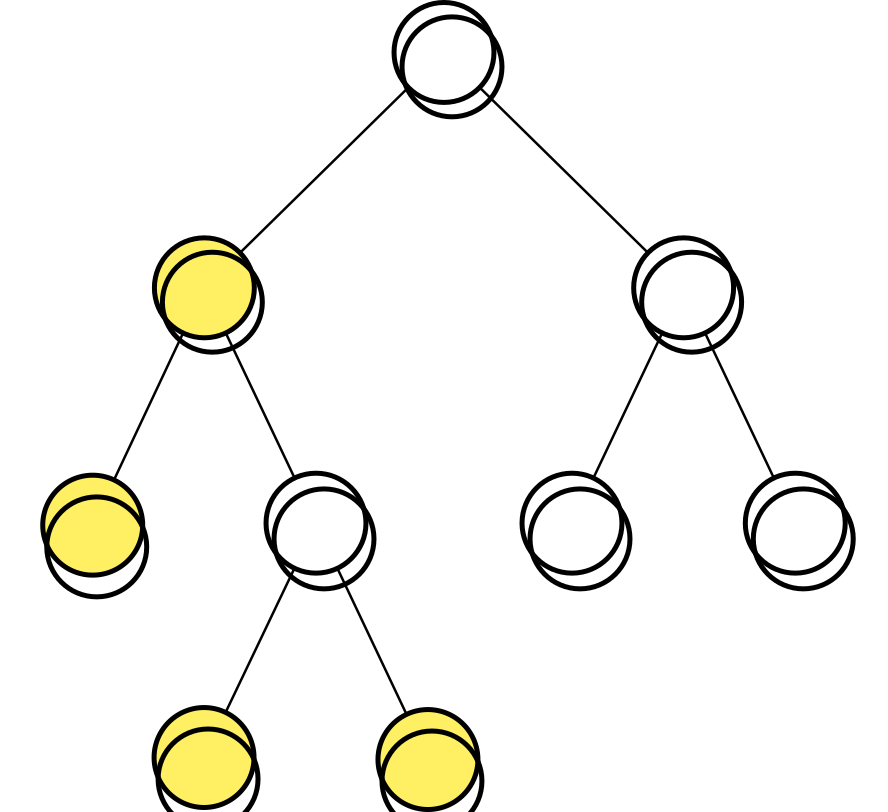
\includegraphics[width=0.3\textwidth]{img/uppaal-tctl-5}
  }
  \caption{Własności TCTL.}
  \label{img:tctl-props}
\end{figure}

% W~celu ułatwienia weryfikacji ilościowej autorzy \upp-a rozszerzyli
% przedstawiony język własności o~zapytania \texttt{sup} i~\texttt{inf}.
% Zapytanie \texttt{sup$\{\varphi\}$: x} daje w~wyniku największą wartość,
% którą może przyjąć zmienna $x$ w~stanie spełniającym predykat $\varphi$.
% Analogicznie, zapytanie \texttt{inf} podaje najmniejszą osiągalną wartość.

\chapter{Język modelowania}
\label{c:lang}
Choć modelowanie systemów czasu rzeczywistego -- w~szczególności
systemów sygnalizacji świetlnej -- przy pomocy automatów czasowych
niesie ze sobą wiele korzyści, może być ono zadaniem skomplikowanym
i~czasochłonnym. Wynika to ze swego rodzaju niskopoziomowości tego
formalizmu. Rozwiązaniem tego problemu jest wprowadzenie
sformalizowanego opisu stanowiącego warstwę pośrednią pomiędzy
rzeczywistym systemem a~reprezentującym go modelem.  Niniejszy
rozdział przedstawia koncepcję prostego języka, służącego do tworzenia
takich właśnie opisów.

Podrozdział \ref{c:lang:req} przedstawia podstawowe wymagania, które
powinien spełniać język formalnego modelowania oraz potencjalne
korzyści wynikające z~jego stosowania, natomiast podrozdział
\ref{c:lang:lang} zawiera opis proponowanej składni i semantyki
takiego języka.

\section{Wymagania i~korzyści}
\label{c:lang:req}

\subsection{Pożądane własności}

Kluczowym wymaganiem stawianym specyfikacji w~prezentowanym języku
modelowania jest możliwość jej automatycznego przekształcenia w~model
w~języku automatów czasowych. Po pierwsze daje to jednoznaczną
semantykę takiego opisu: wątpliwości można rozstrzygnąć, symulując
działanie modelu w~wybranym scenariuszu. Po drugie zaś -- udostępnia
korzyści wynikające z~włączenia do projektu formalnych modeli bez
potrzeby ich ręcznego konstruowania.

Kolejnymi pożądanymi cechami omawianego języka modelowania są prostota
i~wysokopoziomowość. W~celu ich zapewnienia należy zawęzić dziedzinę
języka wyłącznie do systemów sygnalizacji świetlnej, dbając
jednocześnie o~to, aby był on dostatecznie elastyczny, by w~przyjętej
formie można było wyspecyfikować jak najliczniejszy zbiór stosowanych
rozwiązań. Aby ułatwić modelowanie, składnia języka powinna być oparta
na istniejącym aparacie pojęciowym.

\subsection{Oczekiwane korzyści}
\label{ss:lang:req:benefits}
Formalny opis w~języku spełniającym powyższe wymagania powinien
stanowić realną wartość dodaną w~projekcie systemu sygnalizacji
świetlnej. Przede wszystkim, byłby on usystematyzowaną
specyfikacją precyzyjnie określającą sposób jego funkcjonowania. Po
drugie automatyczna generacja modeli pozwoliłaby na szybkie
i~niepodatne na błędy modyfikowanie projektu oraz ponowną weryfikację jego
własności. Formalne opisy oraz wygenerowane modele mogłyby być także
wykorzystywane jako podstawa do wprowadzania własnych rozszerzeń już
na poziomie automatów czasowych.

Zauważmy, że wprowadzenie warstwy pośredniej nie tylko ułatwiłoby
modelowanie automatami czasowymi osobom znającym ten formalizm, ale
także dałoby dostęp do korzyści wynikających z~jego stosowania osobom
z~nim niezaznajomionym.

% Przydaje się także do tego, że czasem chcemy dodać do modelu
% coś co jest potrzebne tylko w~weryfikacji.

\section{Składnia i semantyka}
\label{c:lang:lang}

Proponowany język formalnego modelowania pozwala na specyfikację
dowolnego systemu sygnalizacji świetlnej mieszczącego się w ramach
przedstawionych w rozdziale \ref{c:signals}. Charakterystyka
systemu składa się z~opisów warstw tj. potoków, faz oraz
cyklu. Podział parametrów pomiędzy poszczególne warstwy jest zgodny
z~treścią podrozdziału \ref{ss:signals:actuated:summary}. W
specyfikacji pomijamy wszystkie aspekty, które nie są istotne dla
tworzonych modeli i weryfikowanych własności. Należą do nich w
szczególności kwestie takie jak konkretna liczba i typ urządzeń
sygnalizacyjnych, układ skrzyżowania czy kolizyjność poszczególnych
potoków.

Składnia bazuje formacie YAML\cite{YAML}. Sprawia to, że jest ona
zarówno czytelna dla człowieka jak i~łatwa w~przetwarzaniu
maszynowym. Opis w~każdej warstwie jest po prostu słownikiem wartości
odpowiednich parametrów.

\subsection{Elementy wstępne}
Aby uprościć dalszy opis wprowadzamy następujące pomocnicze typy danych:
\lstset{
  emph={id, user, length, intervals, red_amber, amber,
    red_clear, green, max_green, min_green, gap, movements, hold,
    late, flashing, max_time, phases, rest},
  emph=[2]{constants, movement, phase, cycle},
  emphstyle=[2]\underbar,
  morecomment=[l][\color{light-gray}]{//},
  extendedchars=true,
  texcl=true,
  frame=lines
}
\begin{lstlisting}[caption=Pomocnicze typy danych.]
   mvmt_id  == int[0..m]   // \com{m -- liczba potoków}
   phase_id == int[0..p]   // \com{p -- liczba faz}
   time                    // \com{długość odcinka czasu}
\end{lstlisting}

W~celu skrócenia i~uporządkowania specyfikacji możemy zadeklarować słownik
\url{constants}, którego klucze mogą być potem użyte jako stałe. Mogą
być to zarówno proste wartości jak i~całe podsłowniki danych.

\noindent\begin{minipage}{1.0\linewidth}
\begin{lstlisting}[caption=Słownik stałych.]
constants
   M-TIME: 10
   S-TIME: 5
   NS-INT:
      green:     10
      red_clear: 12
\end{lstlisting}
\end{minipage}

\subsection{Potok ruchu}
Na poziomie potoku definiujemy jego identyfikator, typ uczestnika
ruchu (\texttt{user}) oraz długości poszczególnych interwałów.  Dla
sygnału zielonego o~zmiennej długości określamy parametry
\emph{minimalny zielony} (\texttt{min\_green}) oraz \emph{wydłużenie}
(\texttt{gap}). Jeśli jego długość jest stała, wystarczy proste
określenie typu \texttt{time}\footnote{Standardowo w~sygnalizacji
  wzbudzanej sygnał zielony ma zmienną długość dla pojazdów i~stałą --
dla pieszych. Takie rozwiązanie przedstawiono w~listingu. Oczywiście
nic nie stoi na przeszkodzie, aby potokowi pojazdów także przypisać
stałą długość sygnału zielonego.}.

\noindent\begin{minipage}{1.0\linewidth}
\begin{lstlisting}[caption=Schemat opisu potoku pojazdów.]
movement
   id:     mvmt_id
   user:   VEHICLE
   intervals:
      green:
         min_green: time
         gap:       time
      red_amber: time
      amber:     time
      red_clear: time
\end{lstlisting}
\end{minipage}

\noindent\begin{minipage}{1.0\linewidth}
\begin{lstlisting}[caption=Schemat opisu dla potoku pieszych.]
movement
   id:     mvmt_id
   user:   PEDESTRIAN
   intervals:
      green    : time
      flashing : time
      red_clear: time
\end{lstlisting}
\end{minipage}

\subsection{Faza} Specyfikacja dla fazy obejmuje przede wszystkim jej
unikalny identyfikator oraz listę składających się na nią potoków.
Gdy przynajmniej jeden z~potoków należących do fazy ma zmienną długość
okresu aktywności, należy zdefiniować parametr maksymalny zielony
(\texttt{max\_time}).  Dodatkowo dla faz wielopotokowych zdefiniować
można listy potoków:
\begin{itemize}
  \item dla których stosowana będzie procedura podtrzymania sygnału
  (lista \texttt{hold});
  \item dla których zgłoszenia późne będą -- w~miarę możliwości --
  obsługiwane w~bieżącym okresie aktywności fazy (lista \texttt{late}).
\end{itemize}
\noindent\begin{minipage}{1.0\linewidth}
\begin{lstlisting}[caption=Schemat opisu fazy.]
phase:
   id: phase_id
   movements: list of mvmt_id
   max_time : time
   hold: list of mvmt_id
   late: list of mvmt_id
\end{lstlisting}
\end{minipage}

\subsection{Cykl} Podstawowym elementem definicji cyklu jest
uporządkowana lista faz wchodzących w~jego skład. Dodatkowo określić
należy zachowanie się sygnalizacji w~stanie spoczynku (parametr
\texttt{rest}). Wartością tego parametru może być identyfikator fazy,
która ma być wtedy obsługiwana, bądź stała \texttt{REST-IN-RED},
oznaczająca nadawanie sygnału czerwonego wszystkim potokom.

\noindent\begin{minipage}{1.0\linewidth}
\begin{lstlisting}[caption=Schemat opisu cyklu.]
cycle:
   phases: list of phase_id
   rest: phase_id | REST-IN-RED
\end{lstlisting}
\end{minipage}
  
\subsection{Przykład kompletnej specyfikacji}

Poniższa specyfikacja opisuje proste 4-odnogowe skrzyżowanie.
Cykl składa się z~dwóch faz (patrz \imgr{img:lang-spec-example}):
\begin{itemize}
  \item faza dla pojazdów nadjeżdżających z~północy i~południa (potoki
  0~i 1),
  \item faza dla pojazdów nadjeżdżających ze wschodu i~zachodu oraz
  pieszych (potoki 2, 3~i 4).
\end{itemize}
Zwróćmy uwagę na zastosowanie stałych.
\begin{figure}[ht]
  \centering
  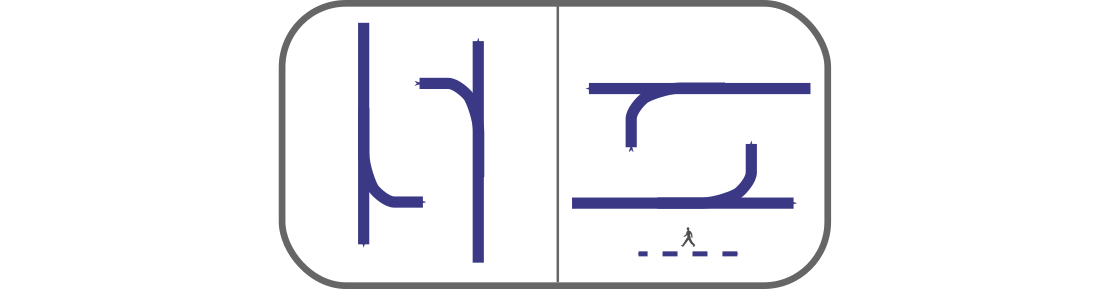
\includegraphics[width=0.5\textwidth]{img/lang-spec-example}
  \caption{Graficzna reprezentacja cyklu opisanego w przykładzie.}
  \label{img:lang-spec-example}
\end{figure}

\begin{lstlisting}[caption=Przykład kompletnej specyfikacji.]
constants
   RED-AMBER: 1
   AMBER:     3
   RED-CLEAR: 4
   NS-INT: // \com{Interwały dla fazy NS}
     green:
       min_green: 6
       gap: 2      
     red_amber: RED-AMBER
     amber:     AMBER
     red_clear: RED-CLEAR
   EW-INT: // \com{Interwały dla fazy EW}
     green:
       min_green: 12
       gap:       3     
     red_amber: RED-AMBER
     amber:     AMBER
     red_clear: RED-CLEAR

movement    // \com{Potok N}
   id: 0    
   user:   VEHICLE
   intervals: NS-INT
movement    // \com{Potok S}
   id: 1    
   user:   VEHICLE
   intervals: NS-INT
movement    // \com{Potok E}
   id: 2   
   user:   VEHICLE
   intervals: EW-INT
movement
   id: 3   // \com{Potok W}
   user:   VEHICLE
   intervals: EW-INT
movement   // \com{Potok pieszy EW}
   id: 4    
   user:   PEDESTRIAN
   intervals:
      green    : 10
      flashing : 3
      red_clear: 5

phase: // \com{Faza NS}
   id: 0
   movements: [0, 1]
   max_time : 12
   hold: [0, 1]
   late: [0, 1]
phase: // \com{Faza EW}
   id: 1
   movements: [2, 3, 4]
   max_time : 20
   hold: [2, 3]
   late: [2, 3]

cycle:
   phases: [0, 1]
   rest: REST-IN-RED
\end{lstlisting}

\chapter{Modele}
\label{c:models}
Kluczową kwestią niezbędną dla osiągnięcia pełni korzyści wymienionych
w~\ref{ss:lang:req:benefits} jest wysoka jakość generowanych
modeli. Niniejszy rozdział przedstawia najważniejsze kwestie związane
z~ich konstrukcją.

Podrozdział \ref{s:models:assumptions} zawiera opis dodatkowych
założeń, które przyjęto, projektując modele. Podrozdział
\ref{s:models:models} przedstawia podział systemu na komponenty, ich
strukturę oraz podstawowy schemat działania, natomiast
\ref{s:models:project} omawia najważniejsze decyzje projektowe.

\section{Założenia}
\label{s:models:assumptions}

Przyjęcie upraszczających rzeczywistość założeń wynika z~samej istoty
modelowania. Ich źródłem mogą być zarówno cechy samego systemu jak
i~formalizm przyjęty jako język modelowania.

Przyjęto następujące założenia o~ruchu pojazdów i~pracy czujników:
\begin{itemize}
  \item Każde zgłoszenie otrzymane w~trakcie interwału zielonego uważa
  się za obsłużone tj. przyjmuje się, że pojazd, od którego pochodzi,
  opuszcza skrzyżowanie. Pominięte zostają scenariusze, w~których
  czujnik zostanie wzbudzony w~trakcie interwału zielonego, lecz
  pojazd nie opuści skrzyżowania.
  \item Każde zgłoszenie przyjęte poza interwałem zielonym będzie
  obsłużone w~przyszłości tj. w~końcu zostanie wyświetlony sygnał
  zielony. Stanie się tak także wtedy, gdy właściwy pojazd opuści
  skrzyżowanie wcześniej. 
\end{itemize}
Formalnym ujęciem powyższych założeń jest następująca własność
żywotności, której spełnienia będziemy oczekiwali od stworzonych
modeli sygnalizacji: przyjęcie zgłoszenia oznacza, że albo sygnał
zielony jest właśnie wyświetlany, albo zostanie on w~końcu
wyświetlony.

Źródłem następnego założenia jest formalizm automatów czasowych. Nie
nakłada on żadnych ograniczeń na czas, który upływa pomiędzy kolejnymi
tranzycjami, co sprawia, że możliwy jest scenariusz, w~którym
nieskończenie wiele tranzycji zostanie wykonanych w~skończonym odcinku
czasu (w szczególności -- zerowym). Modele, w~których on zachodzi,
nazywamy \emph{zenonowskimi} \cite{henz-94}.  Potencjalnie zenonowskie
są w~naszych systemach automaty modelujące zachowanie środowiska
zewnętrznego, czyli czujniki. Aby wykluczyć ich niepożądane biegi, nie
pozwalamy na wzbudzenie czujnika częściej niż co jedną jednostkę czasu
(patrz \imgr{img:models-zeno}). Można to odnieść do rzeczywistości,
uznając, że bardzo bliskie w~czasie wzbudzenia zlepiane są w~jedno.

\begin{figure}
  \centering
  \subfloat[Automat zenonowski.]{
    \includegraphics[height=1in]{img/models-zeno}
  }\hspace{1in}
  \subfloat[Automat niezenonowski.]{
    \includegraphics[height=1in]{img/models-nonzeno}
  }
  \caption{Zenonowskość.}
  \label{img:models-zeno}
\end{figure}

\section{Modele}
\label{s:models:models}
Proponowany model systemu sygnalizacji świetlnej składa się
z~komponentów, będących wydzielonymi jednostkami o~określonej
odpowiedzialności. Rolę komponentu odgrywa jeden bądź dwa ściśle
powiązane automaty czasowe. Wszystkie komponenty można podzielić na
dwie grupy:
\begin{itemize}
  \item komponenty reprezentujące elementy systemu, które biorą udział
  w~interakcji ze środowiskiem zewnętrznym,
  \item komponenty reprezentujące elementy układu sterowania.
\end{itemize}
Do pierwszej grupy należą czujniki i~sygnalizatory, do drugiej zaś --
kontrolery. Dla każdego poziomu opisu systemu, tj. potoku, fazy oraz
cyklu, przewidziano jeden zarządzający nim kontroler.

Sekcja \ref{ss:models:models:summary} prezentuje ogólne informacje
o~pracy komponentów, natomiast sekcje
\ref{ss:models:models:dets}-\ref{ss:models:models:ring} szczegółowo
opisują ich strukturę i~sposób funkcjonowania. Nacisk położony jest w
nich na najbardziej złożone wersje komponentów -- sterujące
sygnalizacją wzbudzaną dla pojazdów; informacje o pozostałych znajdują
się w dodatku \ref{app:other-models}.


\subsection{Ogólny zarys pracy komponentów}
\label{ss:models:models:summary}
Komponenty tworzą strukturę warstwową (patrz \imgr{img:hierarchy}). Do
komunikacji dochodzi w~zasadzie tylko pomiędzy sąsiadującymi
warstwami. Co więcej, jest to struktura hierarchiczna: komponent
wysyła polecenia jednemu bądź większej liczbie swoich komponentów
podrzędnych oraz otrzymuje je od swojego komponentu nadrzędnego.
\begin{figure}[h]
  \centering
  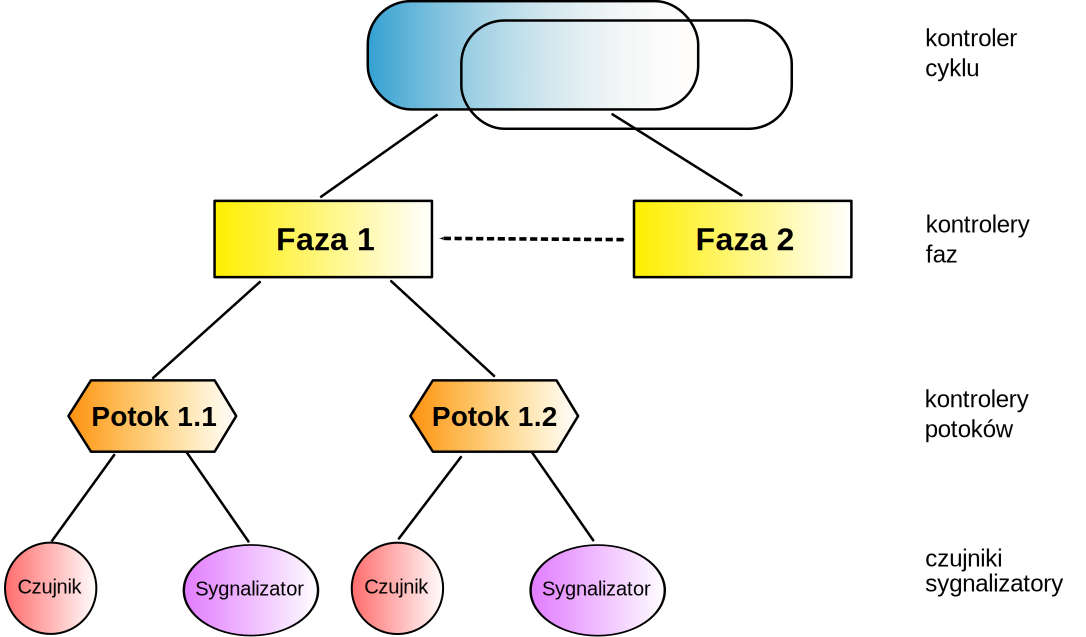
\includegraphics[width=0.9\textwidth]{img/models-hierarchy}
  \caption{Zależności między poszczególnymi komponentami modelu.}
  \label{img:hierarchy}
\end{figure}

Tabela \ref{tab:models:channels} podsumowuje najważniejsze kanały
komunikacyjne modelu, natomiast \imgr{img:models:msc} przedstawia
podstawowy schemat komunikacji.

\renewcommand{\arraystretch}{1.3}
\begin{table}
  \centering
  \begin{tabular}{>{\scshape}r|p{0.35\textwidth}|>{\ttfamily}p{0.25\textwidth}}
    \firsthline\firsthline
    \textbf{Komponenty} & \textbf{Komunikat} & \textnormal{\bfseries Nazwa kanału} \\ \hline
    Czujnik \rarr\ Potok & zgłoszenie & act[mvmt\_id] \\ \hline
    Potok \rarr\ Sygnalizator & polecenie zmiany sygnału & chg[mvmt\_id]
    \\ \hline
    Potok \rarr\ Faza & zgłoszenie zapotrzebowania & call[phase\_id] \\
                      & informacja o~wykryciu luki & gapped\_out[phase\_id] \\
                      & potwierdzenie zakończenia aktywności & gone\_off[phase\_id]
    \\ \hline
    Faza \rarr\ Potok & polecenie startu & go[mvmt\_id] \\
                      & polecenie zakończenia & go\_off[mvmt\_id] \\
                      & osiągnięcie czasu maksymalnego & maxed\_out[phase\_id]
    \\ \hline
    Faza \rarr\ Faza & zgłoszenie przeciwne & opp
    \\ \hline
    Cykl \rarr\ Faza & polecenie startu & start \\ \hline
    Faza \rarr\ Cykl & potwierdzenie zakończenia aktywności & finished \\
    \hline\hline
  \end{tabular}
  \caption{Komunikacja między komponentami.}
  \label{tab:models:channels}
\end{table}

\begin{figure}
  \centering
  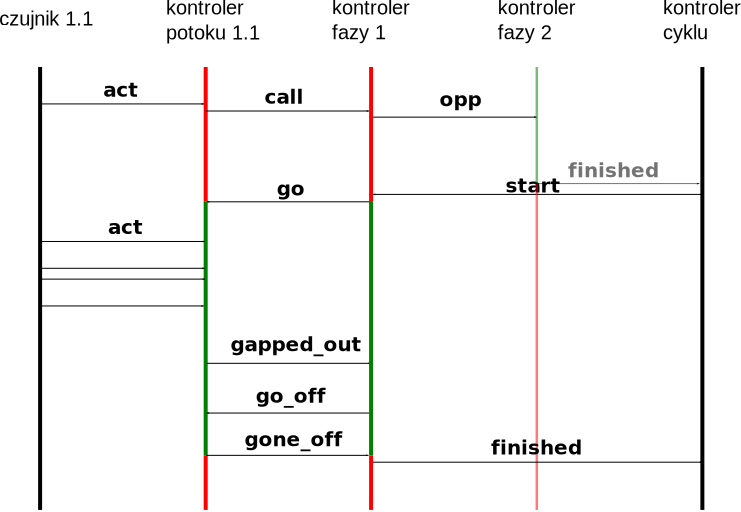
\includegraphics[width=0.8\textwidth]{img/models-msc}
  \caption{Podstawowy schemat komunikacji pomiędzy procesami.}
  \caption*{Schemat przedstawia komunikację w~jednym cyklu aktywności
    fazy. Dla uproszczenia pominięto komunikację kontrolera potoku
    z~sygnalizatorem oraz komunikację między komponentami fazy 2.}
  \label{img:models:msc}
\end{figure}

\subsection{Czujniki i~sygnalizatory}
\label{ss:models:models:dets}
Komponenty należące do najniższej warstwy systemu są prostymi
automatami czasowymi.
Sygnalizatory nie zawierają żadnych elementów sterowania, przyjmują
one jedynie polecenia zmiany sygnału (kanał \url{chg}) od właściwych
kontrolerów potoku (patrz \imgr{img:lights}).

\begin{figure}
  \centering
  \subfloat[Sygnalizator dla pojazdów]{
    \includegraphics[width=0.35\textwidth]{img/models-light-car}
  }
  \hspace{1cm}
  \subfloat[Sygnalizator dla pieszych]{
    \includegraphics[width=0.35\textwidth]{img/models-light-ped}
  }
  \caption{Automaty reprezentujące sygnalizatory.}
  \label{img:lights}
\end{figure}

Czujniki zgłaszają zapotrzebowanie kontrolerom potoku poprzez
komunikat \url{act}. Czujniki dla pojazdów są w~zasadzie automatami
jednostanowymi: w~stanie \url{Actuated} nie upływa czas. Rolę
zegara \url{zeno_t} omówiono w~podrozdziale~\ref{s:models:assumptions}, natomiast
zmiennej \url{service[id]} w~\ref{s:models:opt}. Czujnik dla pieszych
ma natomiast dwa istotne stany, co modeluje zachowanie typowego
przycisku. Zwróćmy uwagę na fakt, że jest on jawnie resetowany
(\url{button_reset}).

\begin{figure}
  \centering
  \subfloat[Czujnik dla pojazdów]{
    \includegraphics[width=0.4\textwidth]{img/models-detector-car}
  }
  \hspace{1cm}
  \subfloat[Czujnik dla pieszych]{
    \includegraphics[width=0.4\textwidth]{img/models-detector-ped}
  }
  \caption{Automaty reprezentujące czujniki.}
  \label{img:detectors}
\end{figure}

\subsection{Kontroler potoku}
Kontroler potoku zarządza pracą pojedynczego sygnalizatora poprzez
decydowanie o~długości wyświetlanych sygnałów (w ramach wyznaczonych
przez odpowiedni kontroler fazy). Odbiera on również zgłoszenia od
odpowiedniego czujnika.

Poniżej znajduje się opis modelu kontrolera w~pełni wzbudzanego potoku
dla pojazdów.
\paragraph{Struktura} Funkcję kontrolera potoku pełni jeden automat
o~następujących parametrach:
\begin{itemize}
  \item \url{id} -- identyfikator potoku;
  \item \url{pid} -- identyfikator fazy, w~skład której wchodzi dany potok;
  \item \url{RED_AMBER}, \url{INIT_GREEN}, \url{AMBER},
  \url{RED_CLEAR}, \url{GAP} -- parametry decydujące o~długości
  poszczególnych sygnałów.
\end{itemize}
Struktura kontrolera potoków jest ściśle związana z~nadawanymi
sygnałami (patrz \imgr{img:mvmt-ctrl}). Mamy zatem stan dla
każdego sygnału o~stałej długości oraz zestaw stanów dla
sygnałów o~zmiennej długości. Wśród stanów ,,zielonych''
wyróżniamy:
\begin{itemize}
  \item \texttt{InitialGreen} -- część początkowa,
  \item \texttt{ExtGreen} -- cześć rozszerzalna przed wykryciem luki,
  \item \texttt{GappedOut} -- cześć rozszerzalna po wykryciu luki,
  \item \texttt{Rest} -- stan spoczynku.
\end{itemize}
Natomiast sygnał czerwony związany jest z~następującymi stanami:
\begin{itemize}
  \item \texttt{RedClear} -- okres czyszczenia;
  \item \texttt{RedNoDemand} -- potok nieaktywny, brak zgłoszenia;
  \item \texttt{RedWaiting} -- potok nieaktywny, przyjęto zgłoszenie
  od czujnika.
\end{itemize}
Praca kontrolera potoku nadzorowana jest przez dwa zegary:
\begin{itemize}
  \item \texttt{fixed\_t} -- odpowiada za interwały (bądź ich części)
  o~stałej długości,
  \item \texttt{gap\_t} -- odpowiada za długość części rozszerzalnej
  interwału zielonego; w~momencie otrzymania zgłoszenia jest on
  resetowany, zatem osiągnięcie przezeń wartości równej wydłużeniu
  oznacza wykrycie luki.
\end{itemize}
\paragraph{Bazowy schemat funkcjonowania} Podstawowy cykl pracy
kontrolera potoku wzbudzanego przebiega następująco:
\begin{enumerate}
  \item Kontroler otrzymuje zgłoszenie od czujnika (\texttt{act?}) i~przekazuje
  informację o~zapotrzebowaniu do kontrolera fazy (\texttt{call!}).
  \item Kontroler odbiera polecenie startu od kontrolera fazy
  (\texttt{go?}) i~przechodzi w~stan aktywności.
  \item Kontroler zarządza nadanie sygnału czerwono-żółtego,
  a~następnie części początkowej sygnału zielonego (\texttt{chg!}).
  \item Po zakończeniu części początkowej, kontroler przechodzi do
  części rozszerzalnej; trwa ona aż do momentu, w~którym zajdzie jeden
  z~dwóch warunków:
  \begin{itemize}
    \item zostanie wykryta luka tj. zegar \url{gap_t} osiągnie wartość
    \url{GAP}; informacja o~tym jest wysyłana do kontrolera fazy
    (\url{gapped_out!});
    \item kontroler fazy wyśle informację o~osiągnięciu czasu
    maksymalnego (\texttt{maxed\_out?}).
  \end{itemize}
  \item Kontroler zarządza kolejno nadanie sygnału żółtego
  i~czerwonego-czyszczącego (\texttt{chg!}), po czym zgłasza zakończenie pracy
  kontrolerowi fazy (\texttt{gone\_off!}).
\end{enumerate}

\begin{sidewaysfigure}
  \centering
  \includegraphics[width=0.9\textwidth]{img/models-mvmt}
  \caption{Model kontrolera potoku dla pojazdów.}
  \label{img:mvmt-ctrl}
\end{sidewaysfigure}

\subsection{Kontroler fazy}
\label{ss:models:models:phase-ctrl}
Kontroler fazy zarządza funkcjonowaniem zależnych od siebie
kontrolerów potoków, wyznaczając początek i~maksymalny czas ich pracy.

Poniżej opisano model wielopotokowego kontrolera fazy.
\paragraph{Struktura} Kontroler fazy składa się z~dwóch
automatów. Pierwszy z~nich odpowiada za logikę, zaś drugi wyłącznie za
odmierzanie czasu maksymalnego. Główny automat komunikuje się
z~automatem-zegarem wysyłając mu polecenia \url{timer_on}
i~\url{timer_off}. Podział komponentu na dwie części pozwolił na
zmniejszenie liczby stanów i~ogólne uproszczenie jego struktury.

Główna część kontrolera fazy jest automatem o~następujących
parametrach:
\begin{itemize}
  \item \url{id} -- identyfikator fazy;
  \item \url{m1}, \url{m2}, ... -- identyfikatory składających się na
  nią potoków;
  \item \url{MAX} -- maksymalny zielony.
\end{itemize}
Tak jak w~typowym automacie reprezentującym układ sterujący, większość jej
stanów jest oznaczonych jako uprzywilejowane; do pozostałych należą:
\begin{itemize}
  \item \url{Inactive} -- faza nieaktywna, brak zapotrzebowania;
  \item \url{InactiveWaiting} -- faza nieaktywna, oczekiwanie na
  polecenie startu;
  \item \url{Active} -- faza aktywna;
  \item \url{GoingOff} -- oczekiwanie na potwierdzenia zakończenia
  pracy przez potoki.
\end{itemize}
W~skład konfiguracji kontrolera fazy wchodzą także następujące zmienne:
\begin{itemize}
  \item \url{mvmts_on : int} -- liczba aktywnych potoków,
  \item \url{mvmts_not_out : int} -- liczba potoków, w~których nie wykryto luki,
  \item \url{call_arr[mvmts] : bool} -- dane o~zapotrzebowaniu,
  \item \url{held[mvmts] : bool} -- dane o~podtrzymanych sygnałach,
  \item \url{timer_set : bool} -- informacja o~aktywności zegara czasu
  maksymalnego.
\end{itemize}

\paragraph{Bazowy schemat działania} Podstawowy cykl funkcjonowania
kontrolera przebiega następująco:
\begin{enumerate}
  \item Kontroler przyjmuje zgłoszenie od jednego z~potoków (\url{call?})
  i~przekazuje informację o~zgłoszeniu przeciwnym kontrolerowi aktywnej
  fazy lub kontrolerowi cyklu w~przypadku spoczynku w~czerwonym (\url{opp!}).
  \item Kontroler otrzymuje polecenie startu od kontrolera cyklu
  (\url{start?}) i~przekazuje je tym kontrolerom potoków, które
  zgłosiły zapotrzebowanie (\url{go!}). Jeśli już w~tym momencie jest
  zapotrzebowanie przeciwne, uruchamiany jest zegar czasu
  maksymalnego.
  \item Kontroler przechodzi do~głównego stanu aktywności, w~którym obsługuje
  następujące komunikaty od kontrolerów potoków:
  \begin{itemize}
    \item informacje o~wykryciu luki (\url{gapped_out?}),
    \item informacje o~zakończeniu pracy (\url{gone_off?}),
    \item zgłoszenia późne (\url{call?}).
  \end{itemize}
  Konkretne działanie podejmowane w~każdym z~powyższych przypadków
  zależą od wybranych opcji. Jeśli zgłoszenie przeciwne
  (\url{opp?}) nie zostało obsłużone wcześniej, to może zostać
  obsłużone w~tym stanie tj. uruchomiony będzie zegar czasu
  maksymalnego.
  \item Aktywność fazy może zostać zakończona z~dwóch powodów:
  \begin{itemize}
    \item każdy z~kontrolerów przekazał informację o~wykryciu luki
    (\url{mvmts_not_out == 0}) bądź o~zakończeniu pracy
    (\url{mvmts_on == 0}),
    \item osiągnięty został czas maksymalny.
  \end{itemize}
  W~chwili wystąpienia jednego z~tych warunków kontroler przechodzi
  do~ostatniego etapu swojej pracy. Wysyła wszystkim potokom, które nadal
  wyświetlają sygnał zielony (w szczególności -- podtrzymanym)
  polecenie zakończenia pracy (\url{go_off!}) i~czeka na otrzymanie
  potwierdzenie jego wykonania (\url{gone_off?}). Następnie przechodzi
  do~jednego ze stanów nieaktywności, informując o~tym kontroler cyklu
  (\url{finished!}).
\end{enumerate}

\begin{sidewaysfigure}
  \centering
  \includegraphics[width=1.1\textwidth]{img/models-phasectrl}
  \caption{Model kontrolera fazy (składającej się z~dwóch w~pełni wzbudzanych potoków dla pojazdów).}
  \label{img:phase-ctrl}
\end{sidewaysfigure}

\subsection{Kontroler cyklu}
\label{ss:models:models:ring}
Kontroler cyklu jest najprostszym z~przedstawionych elementów
sterowania sygnalizacją (patrz \imgr{img:ring-ctrl}). Jego jedynym
parametrem jest \url{rest_ph} -- identyfikator fazy spoczynkowej.

Kontroler cyklu uruchamia pierwszą kolejności fazę, na którą
jest zapotrzebowanie (\url{start!}), następnie zaś czeka na
potwierdzenie zakończenia jej aktywności (\url{finished?}). Gdy nie ma
zapotrzebowania na żadną fazę, kontroler przechodzi w~stan spoczynku
bądź uruchamia fazę spoczynkową.

\begin{figure}
  \centering
  \includegraphics[width=0.6\textwidth]{img/models-ring}
  \caption{Model kontrolera cyklu}
  \label{img:ring-ctrl}
\end{figure}

\section{Decyzje projektowe}
\label{s:models:project}

Sposób konstrukcji modelu wynika nie tylko z~samej istoty postawionego
zadania, lecz także z~pewnych ogólnych zasad inżynierii
oprogramowania. Podjęte decyzje projektowe wynikają z~dążenia do
osiągnięcia następujących własności modelu:
\begin{enumerate}
  \item możliwie dokładne odzwierciedlenie funkcjonowania docelowego systemu,
  \item konfigurowalność,
  \item utrzymywalność i~czytelność,
  \item weryfikowalność.
\end{enumerate}
Konstrukcja automatów przebiegała w~dwóch etapach. W~pierwszym,
kierując się głównie założeniami 1-3, przygotowano ogólną strukturę
modelu oraz wstępne wersje poszczególnych automatów. Następnie, o~ile
dostępne zasoby nie pozwalały na weryfikację oczekiwanych własności,
automaty były optymalizowane.

\subsection{Wstępna konstrukcja modelu}

W~pierwszym etapie pracy system został podzielony na komponenty,
określono ich odpowiedzialności oraz interfejsy, przy pomocy których
komunikują się z~pozostałymi. Kierowano się przede wszystkim ogólnie
znanymi zasadami prawidłowego projektowania oprogramowania takimi jak
ukrywanie wewnętrznej implementacji komponentów czy unikanie
powtarzania się podobnych elementów struktury. Już na tym etapie
należało zadbać o~wydajność weryfikacji, co polegało m.in. na
minimalizacji liczby zmiennych (przede wszystkim -- zegarowych) oraz
oznaczaniu stanów jako uprzywilejowane.

\subsection{Optymalizacja modeli}
\label{s:models:opt}

Celem optymalizacji modelu jest redukcja zasobów, tj. pamięci
operacyjnej i~czasu procesora, potrzebnych do zweryfikowania pewnych
jego własności. Kompendium informacji na temat optymalizacji modeli w
\upp-u można odnaleźć w \cite{tutorial04}.

Poniżej przedstawiono najważniejsze z~zastosowanych metod.

\paragraph{Minimalizacja liczby przeplotów} Podstawowym środkiem
służącym optymalizacji modelu jest minimalizacja liczby możliwych
przeplotów i~-- co za tym idzie -- zmniejszenie przestrzeni stanów
przeszukiwanej w~czasie weryfikacji\footnote{Znaczenie ograniczania
  liczby przeplotów jest tym większe, że w~\upp-u nie zaimplementowano
  redukcji częściowo-porządkowych.}. Najprostszą metodą osiągnięcia
tego celu jest wspomniane wyżej oznaczanie stanów jako uprzywilejowane.
Innym sposobem jest uniemożliwienie wykonania tranzycji, które nie
mają znaczenia z~punktu widzenia funkcjonowania docelowego
systemu. Przykładem tego działania było pominięcie nieistotnych,
tj. niemających wpływu na pracę kontrolera, wzbudzeń czujnika. Należą
do nich m.in. wzbudzenia w~początkowej części interwału zielonego lub
wzbudzenia dla nieaktywnego potoku, gdy już wcześniej zostało
zgłoszone zapotrzebowanie. Aby je wyeliminować, dla każdego potoku
wprowadzono zmienną boolowską \url{service}. Kontroler ustawia
jej wartość na prawdziwą, gdy wzbudzenia czujnika są istotne oraz
fałszywą -- w~przeciwnym przypadku. W~automacie reprezentującym
czujnik dodano ograniczenie na krawędź, pozwalające mu przejść w~stan
wzbudzenia wyłącznie wtedy, gdy \url{service} ma wartość prawdziwą.

\paragraph{Redukcja zmiennych aktywnych} Kolejną ważną metodą
optymalizacji modeli jest \emph{redukcja zmiennych aktywnych}.
Chociaż wartości wszystkich zmiennych są stale utrzymywane w~modelu,
czasem zachodzi sytuacja, w~której w~pewnych stanach wartość
niektórych z~nich nie ma znaczenia: dwie konfiguracje różniące się wyłącznie
takimi zmiennymi można uznać za identyczne. Zresetowanie wartości tych
zmiennych utożsami zatem te konfiguracje, co zmniejszy rozmiar przeszukiwanej
przy weryfikacji przestrzeni.

Powyższe rozważania formalizuje następująca definicja: zmienną $v$
nazywamy \emph{nieaktywną} w~stanie $l$, gdy na wszystkich
ścieżkach zaczynających się w~$l$, $v$ zostanie zresetowana zanim
zostanie odczytana. Jeśli zmienna $v$ jest nieaktywna w~stanie
$l$ należy zresetować jej wartość na wszystkich krawędziach
prowadzących do $l$. Wyjątkiem jest sytuacja, w~której $v$ jest
nieaktywna już we wszystkich stanach, z~których prowadzą
krawędzie do $l$. Znaczy to, że jej wartość została zresetowana już wcześniej
i~nie ma potrzeby powtarzania tej operacji.

\upp\ przeprowadza analizę aktywności zmiennych zegarowych w~trakcie
weryfikacji, zatem zasadniczo nie ma potrzeby ręcznego resetowania
nieaktywnych zmiennych. Niestety automatyczna analiza często zawodzi
w~przypadku, gdy mamy do czynienia z~tablicami zegarów. Dlatego też
w~automacie odmierzającym czas maksymalny, wprowadzono jawne resetowanie
zegarów (patrz \imgr{img:models-active-reduction}).

\begin{figure}
  \centering
  \subfloat[Zegar czasu maksymalnego bez jawnej redukcji nieaktywnej zmiennej.] {
    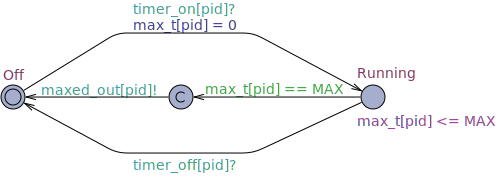
\includegraphics[width=0.45\textwidth]{img/models-maxtimer-noactred}
  }\hfill
  \subfloat[Zegar czasu maksymalnego z~jawną redukcją nieaktywnej zmiennej.] {
    \includegraphics[width=0.45\textwidth]{img/models-maxtimer}
  }
  \caption{Redukcja zmiennych aktywnych}
  \label{img:models-active-reduction}
\end{figure}

\paragraph{Abstrakcja} Zaproponowane wyżej metody optymalizacji modeli
nie powodują zmniejszenia dokładności, z~jaką reprezentowany jest
docelowy system. Często okazują się one jednak niewystarczające, aby
móc dowieść jego pożądanych własności. Należy wtedy uprościć model,
rezygnując z~reprezentowania tych cech systemu, które są nieistotne
dla danej własności.

Przykładem takiego uproszczenia jest pominięcie nadawania sygnałów
czerwono-żółtego i~żółtego. Metoda ta została zastosowana przy
weryfikacji najbardziej skomplikowanych systemów.
% Jako, że są one
% zarządzane wyłącznie przez kontroler potoku, taka abstrakcja nie
% powinna mieć na wpływu własności dotyczące poprawnej współpracy
% komponentów systemu.

\chapter{Eksperymenty}
\label{c:ver}
Możliwość automatycznej weryfikacji pożądanych własności
projektowanego systemu jest główną przyczyną, dla której korzysta się
z metod formalnych. Niniejszy rozdział omawia najważniejsze kwestie
związane z weryfikacją przedstawionych wcześniej modeli sygnalizacji
świetlnej. Jego celem jest z~jednej strony wykazanie, że są one
zaprojektowane prawidłowo; z~drugiej zaś zaprezentowanie sposobu,
w~jaki korzystać z nich może użytkownik.

Podrozdział \ref{s:ver:properties} prezentuje najważniejsze
z~weryfikowanych własności, natomiast podrozdział \ref{s:ver:results}
omawia wyniki weryfikacji.

\section{Weryfikowane własności}
\label{s:ver:properties}

Pożądane własności systemu można podzielić na dwie grupy. Do pierwszej
należą własności bezpieczeństwa, tj. te, które stwierdzają, że
wszystkie osiągalne konfiguracje są prawidłowe. Do drugiej zaś
własności żywotności -- mówiące o realizacji każdego żądania.

\subsection{Podstawowe własności bezpieczeństwa}
\label{s:ver:properties:safety}

\paragraph{Brak zakleszczenia} Własność braku zakleszczenia,
tj. możliwość wykonania dopuszczalnej tranzycji w~każdym osiągalnym
stanie systemu, jest kluczowa dla poprawności każdego systemu czasu
rzeczywistego. W~\upp-u wyrażana jest ona poprzez formułę:
\begin{center}
  \url{A[] not deadlock}
\end{center}

\paragraph{Poprawna współpraca kontrolerów}
Zauważmy, że już brak zakleszczeń w~modelu daje nam pewne informacje
o~poprawności współpracy poszczególnych komponentów. Rozpatrzmy często
powtarzający się element struktury automatów, jakim jest stan uprzywilejowany,
którego opuszczenie wiąże się z~synchronizacją na pewnym kanale
komunikacyjnym. Brak blokady w~takim stanie oznacza, że
komunikacja może odbyć się natychmiast, co z~kolei świadczy
o~zgodności stanów automatów będących jej stronami. Przykładem takiej
sytuacji jest brak zakleszczenia w stanie \url{Actuated} czujnika,
z którego można wywnioskować, że wszystkie wzbudzenia są natychmiast obsługiwane
przez kontroler potoku.

Dalsze informacje o~poprawności współpracy poszczególnych komponentów
możemy uzyskać weryfikując m.in. następujące formuły:

\begin{itemize}
  \item Zgodność stanu kontrolera potoku (\url{MvC}) i~sygnału
  wyświetlanego przez sygnalizator (\url{L}):\\
  \url{A[] (MvC.InitGreen||MvC.ExtGreen||MvC.GappedOut||MvC.Rest) imply L.Green}\\
  \url{A[] (MvC.RedClear||MvC.RedNoDemand||MvC.RedWaiting) imply L.Red}\\
  \url{A[] MvC.RedAmber imply L.RedAmber}\\
  \url{A[] MvC.Amber imply L.Amber}
  \item Zgodność stanu kontrolera potoku (\url{MvC00}) i~kontrolera
  fazy (\url{PC0}):\\
  \url{A[] PC0.Inactive imply (MvC00.RedNoDemand||MvC00.RedGotCall)}\\
  \url{A[] (PC0.InactiveWaiting && call_arr[0]) imply MvC00.RedWaiting}\\
  \url{A[] (PC0.InactiveWaiting && not call_arr[0]) imply MvC00.RedNoDemand}
  \item Zgodność stanu kontrolera fazy (\url{PC0}) i~kontrolera cyklu
  (\url{Ring}): \\
  \url{A[] PC0.Active imply (Ring.Active && Ring.cur == 0)}
\end{itemize}

\paragraph{Bezpieczeństwo pracy sygnalizacji}
Funkcjonowanie systemu sygnalizacji świetlnej jest bezpieczne, gdy
kolidujące potoki ruchu są segregowane w~czasie tj. nie są aktywne w
tym samym czasie. Pierwszym pomysłem na wyrażenie tej własności w
naszych modelach są formuły typu:
\begin{center}
\ttt{A[] Light00.Green imply Light10.Red}\\
\ttt{A[] Light00.Amber imply Light10.Red}\\
\ttt{...}
\end{center}
gdzie \ttt{Light00} i \ttt{Light10} są modelami reprezentującymi
sygnalizatory kolidujących potoków. Wykorzystując fakt, że kolidujące
potoki należą do różnych faz możemy wyrazić tę własność zwięźlej,
mówiąc, że w danym momencie aktywna jest co najwyżej jedna faza. Dla
systemu dwufazowego opisuje to poniższa formuła:
\begin{center}
  \url{A[] PC0.Active + PC1.Active <= 1}
\end{center}
Biorąc pod uwagę fakt, że na mocy wcześniej wymienionych własności,
nieaktywność fazy oznacza wyświetlanie sygnału czerwonego dla
wszystkich jej potoków, powyższa formuła daje nam pożądaną własność
bezpieczeństwa.

% W~silniejszym wariancie bezpieczeństwa, można wymagać nie tylko, aby
% kolidujące potoki nie otrzymywały jednocześnie sygnału zielonego, ale
% by ich zielone interwały były oddzielone dostatecznie długimi
% interwałami przejściowymi. Weryfikacja takiej własności wymaga
% rozszerzenia modelu o~zmienną \url{finished} ustawianą na true dodatkowy zegar \url{safe_t} resetowany
% w~momencie kończenia...

\subsection{Żywotność}
\label{s:properties:liveness}

Żywotność systemu sygnalizacji wzbudzanej oznacza, że każde zgłoszenie
zostanie obsłużone tj. odpowiedni sygnalizator zezwoli na opuszczenie
skrzyżowania każdemu uczestnikowi ruchu. W~przedstawionych modelach
własność tę wyraża następująca formuła:
\tttform{A[] Detector.Actuated --> Light.Green}
Zauważmy jednak, że w~analizie systemów czasu rzeczywistego przeważnie
interesuje nas nie tylko sam fakt obsłużenia żądania, ale także
długość odcinka czasu między żądaniem a~jego realizacją. Stosowna
własność nazywa się ograniczoną żywotnością \ang{bounded liveness}
i~definiuje w~następujący sposób:

\begin{definition}[Ograniczona żywotność]
  System spełnia własność ograniczonej żywotności $\varphi
  \leadsto_{\leq t} \psi $ wtedy i~tylko wtedy, gdy po każdej
  konfiguracji, w~której prawdziwy jest predykat $\varphi$, nie
  później niż po $t$ jednostkach czasu, nastąpi konfiguracja, w~której
  prawdziwy jest predykat~$\psi$.
\end{definition}
Najprostszym sposobem weryfikacji tak zdefiniowanej żywotności byłoby
dodanie zegara $z$ resetowanego ilekroć stan automatu zaczyna
spełniać $\varphi$ i~weryfikowanie własności \mbox{$\varphi \leadsto
  (\psi \land z\leq t)$}. Dalece bardziej efektywna metoda, polegająca
na sprowadzeniu żywotności ograniczonej do prostej własności
bezpieczeństwa, została zaproponowana w~\cite{lpw:tacas98}. Aby ją
zastosować należy, obok dodatkowego zegara, rozszerzyć model o~zmienną
boolowską $b$, zainicjowaną na $false$.  W~momencie, gdy predykat
$\varphi$ zaczyna być spełniony, $b$ jest ustawiana na $true$ a~zegar
$z$ jest resetowany; wartość $false$ jest przypisywana z~powrotem na
$b$, gdy tylko zajdzie predykat $\psi$. Zmienna $b$ przechowuje zatem
informację, o~tym czy mamy do czynienia z~aktywnym żądaniem spełnienia
$\psi$.

Rolę zmiennej $b$ w modelu pełni zmienna \ttt{v_demand} będąca składową
kontrolera potoku, a zegara $z$ -- \ttt{wait_t}. Wartość \ttt{v_demand}
jest ustawiana na $true$ w momencie otrzymania zgłoszenia, a na
$false$ -- w momencie włączenia sygnału zielonego. Końcowa wersja
formuły wygląda następująco:
\tttform{A[] MvmtCtrl.v_demand imply MvmtCtrl.wait_t <= MAX_WAIT}
Aby otrzymać ostre ograniczenie górne na długość oczekiwania należy
znaleźć taki parametr \ttt{MAX_WAIT}, dla którego powyższa formuła
jest prawdziwa, natomiast jej wersja z~ostrą nierównością -- nie jest.

\section{Wyniki weryfikacji}
\label{s:ver:results}
\subsection{Parametry sprzętowe i oprogramowanie}
Eksperymenty przeprowadzono na komputerze o następującej konfiguracji
sprzętowej i programowej:
\begin{itemize}
  \item procesor: Intel Core i3, 2,93GHz;
  \item pamięć operacyjna: 4GB;
  \item system operacyjny: Ubuntu Linux 64-bit, wersja jądra 2.6.38. 
\end{itemize}
Wykorzystany został \upp\ w wersji 4.1.3 (4577).

\subsection{Weryfikacja podstawowych własności.}
Niniejszy rozdział prezentuje wyniki weryfikacji poniższych formuł:
\begin{enumerate}
  \item \ttt{A[] PC0.Inactive imply (MvC00.RedNoDemand||MvC00.RedGotCall)}
  \item \ttt{A[]
  (MvC00.InitGreen||MvC00.ExtGreen||MvC00.GappedOut||MvC00.Rest) imply
  L00.Green}
  \item Dla modelu A: \ttt{A[] (PC0.Active + PC1.Active + PC2.Active
    <= 1)}\\
  Dla modelu B: \ttt{A[] (PC0.Active + PC1.Active + PC2.Active +
    PC3.Active <= 1)}
  \item \ttt{A[] (MvC00.v_demand imply MvC00.wait_t <= MAX_WAIT)}
  \item \ttt{A[] (MvC00.v_demand imply MvC00.wait_t < MAX_WAIT)}
  \item \ttt{A[] not deadlock}
  \item \ttt{Detector00.Actuated --> Light00.Green}
\end{enumerate}

W eksperymentach zastosowano dwa z dostępnych w \upp-u trybów
reprezentacji przestrzeni konfiguracji:
\begin{itemize}
  \item zwarta struktura danych \ang{compact data structure} -- ustawienie domyślne,
  \item nadaproksymacja -- przybliżenie konfiguracji z góry, polegające na
  znajdowaniu otoczki wypukłej stref.
\end{itemize}
Druga z wymienionych opcji jest bardzo cenna w weryfikacji własności
bezpieczeństwa, jako że powoduje istotne zmniejszenie przeszukiwanej
przestrzeni konfiguracji. Ustawienie jej sprawia jednak, że
weryfikator może nie być w stanie udzielić pełnej -- twierdzącej bądź
przeczącej -- odpowiedzi dla niektórych formuł, np. braku zakleszczenia.

Eksperymenty przeprowadzono dla dwóch modeli sygnalizacji dla prostych
skrzyżowań. Składają się one wyłącznie z potoków dla pojazdów o
identycznych parametrach. Formalne opisy weryfikowanych modeli można
odnaleźć w dodatku \ref{app:descriptions}.

\paragraph{Model A} Model A reprezentuje sygnalizację dla skrzyżowania
4-odnogowego, na którym pojazdy nadjeżdżające z północy oraz południa
mają zapewniony bezkolizyjny przejazd. Cykl pracy systemu składa się z
trzech faz zaprezentowanych na \imgr{img:ver-phases-a}.

\begin{figure}[ht]
  \centering
  
\includegraphics[width=0.5\textwidth]{img/ver-a-cycle}
  \caption{Fazy modelu A}
  \label{img:ver-phases-a}
\end{figure}
\begin{table}[ht]
  \centering
  \begin{tabular}{|r||r|r|r||r|r|r||}
    \hline
    & \multicolumn{3}{c||}{\bf Standard} & \multicolumn{3}{c||}{\bf
      Otoczka wypukła} \\ \hline
    Nr   & Wynik & Czas [min:s] & Liczba stanów & Wynik & Czas [min:s] &
    Liczba stanów \\ \hline
    1. & TAK & 0:23   &  325~708 & TAK & 0:09 & 223~909 \\
    2. & TAK & 0:23   &  325~708 & TAK & 0:09 & 223~909 \\
    3. & TAK & 0:31   &  325~708 & TAK & 0:09 & 223~909 \\
    4. & TAK & 4:08   & 1~578~972 & TAK & 0:43 & 939~842 \\
    5. & NIE & 3:02   & 1~190~193 & ?   & 0:34 & 752~817 \\
    6. & TAK & 102:40 & 3~067~518 & ?   & 0:12 & 166~794 \\
    7. & TAK & 941:16 & 3~067~438 & ?   & $<$0:01   &     b/d  
    \\\hline
  \end{tabular}
  \caption{Statystyki z weryfikacji dla modelu A.}
  \caption*{Znaki zapytania oznaczają odpowiedź: \emph{Własność może
      nie być prawdziwa}. Zwróćmy uwagę na bardzo długi czas potrzebny
  do zweryfikowania pełnej żywotności.}
  \label{tab:ver-stats-a}
\end{table}

\paragraph{Model B} Model B reprezentuje sygnalizację dla
skrzyżowania, na którym wszystkie pojazdy mają zapewniony bezkolizyjny
przejazd. Cykl pracy systemu składa się z czterech faz
zaprezentowanych na \imgr{img:ver-phases-b}.

\begin{figure}
  \centering
  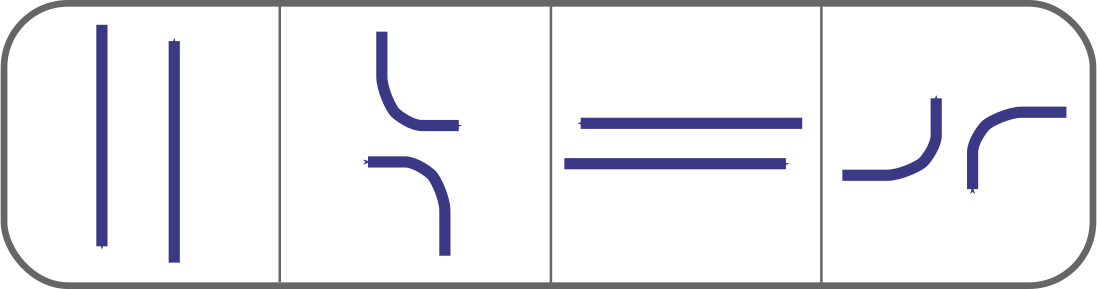
\includegraphics[width=0.5\textwidth]{img/ver-b-cycle}
  \caption{Fazy modelu B}
  \label{img:ver-phases-b}
\end{figure}
\begin{table}[ht]
  \centering
  \begin{tabular}{|r||r|r|r||r|r|r||}
    \hline
    & \multicolumn{3}{c||}{\bf Standard} & \multicolumn{3}{c||}{\bf
      Otoczka wypukła} \\ \hline
    Nr   & Wynik & Czas [min:s] & Liczba stanów & Wynik & Czas [min:s] &
    Liczba stanów\\ \hline
    1. & TAK &  7:58 & 3~017~585  & TAK  & 2:09  &  1~929~817 \\
    2. & TAK &  8:44 & 3~017~585  & TAK  & 2:08  &  1~929~817 \\
    3. & TAK & 10:16 & 3~017~585  & TAK  & 2:03  &  1~929~817 \\
    4. & TAK & 59:44 & 16~664~531 & TAK  & 10:03 & 10~043~278 \\
    5. & NIE & 43:54 & 13~757~176 & ?    & 7:31  &  8~631~811 \\
    6. & --  & 6000:00 & b/d            & ?    & 2:20  &  1~549~044 \\
    7. & --  & 6000:00 & b/d         & ?    & 0:01  &       b/d 
    \\\hline
  \end{tabular}
  \caption{Statystyki z weryfikacji dla modelu B.}
  \caption*{Znaki zapytania oznaczają odpowiedź: \emph{Własność może
      nie być prawdziwa}. Kreski oznaczają, że danej formuły nie udało
  się zweryfikować w podanym czasie.}
  \label{tab:ver-stats-b}
\end{table}
\subsection{Parametry modelu a~zasoby potrzebne do weryfikacji jego
  własności}
Statystyki przedstawione w poprzednim podrozdziale wyraźnie pokazują,
że kluczowym czynnikiem mającym wpływ na zasoby potrzebne do
weryfikacji jest rozmiar modelu rozumiany jako liczba faz i
potoków. Rolę odgrywają jednak także pozostałe parametry takie jak
np. maksymalny zielony.  Wpływ tego parametru na czas weryfikacji i
liczbę przejrzanych stanów prezentuje \imgr{img:max-time-chart}. W
eksperymencie wykorzystano model A, zmieniając tylko odpowiednio
pararametr maksymalny zielony (dla wszystkich faz). Weryfikowano
własność \ttt{A[] not deadlock}.
\begin{figure}
  \centering
  \subfloat[Czas weryfikacji.]{
    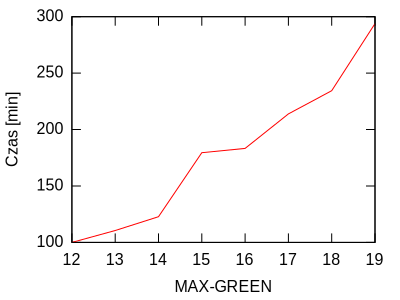
\includegraphics[width=0.6\textwidth]{img/ver-max-time-chart}
  }\\
  \subfloat[Liczba przejrzanych konfiguracji.]{
    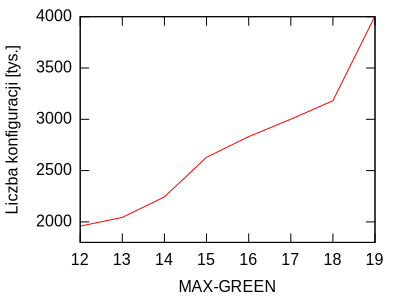
\includegraphics[width=0.6\textwidth]{img/ver-max-states-chart}
  }
  \caption{Zależność zasobów potrzebnych do weryfikacji od parametru maksymalny zielony.}
  \label{img:max-time-chart}
\end{figure}

Wzrost rozmiaru przestrzeni konfiguracji wraz ze wzrostem czasu
maksymalnego nie stoi w sprzeczności z uwagą z rozdziału
\ref{ss:ta:theory:verification} o niezależności stref od
konkretnych wartości stałych w ograniczeniach. Zauważmy bowiem, że
zwiększenie omawianego parametru powoduje istotny wzrost liczby
możliwych scenariuszy -- w każdym odcinku aktywności fazy czujniki
mogą być wzbudzone więcej razy.

%%%%%%%%%%%%%%%%%%%%%%%%%%%%%%%%%%%%%%%%%%%%%%%%%%%%%%%%%%%%%%%%%%%%%
% Koniec zasadniczej części pracy
%%%%%%%%%%%%%%%%%%%%%%%%%%%%%%%%%%%%%%%%%%%%%%%%%%%%%%%%%%%%%%%%%%%%%
\appendix
\chapter{Modele pozostałych komponentów}
\label{app:other-models}

\section{Kontroler potoku}
\paragraph{Model kontrolera potoku dla pieszych} Struktura i schemat
funkcjonowania kontrolera potoku dla pieszych są podobne do tych dla
jego odpowiednika dla potoku pojazdów. Uproszczenia wynikają z
mniejszej liczby nadawanych sygnałów oraz z faktu, że sygnał zielony
ma stałą długość (stąd tylko jeden ,,zielony'' stan). Patrz
\imgr{img:models-extra:pedctrl}.
\begin{figure}[ht]
  \includegraphics[width=\textwidth]{img/models-pedctrl}
  \caption{Automat reprezentujący kontroler potoku dla pieszych.}
  \label{img:models-extra:pedctrl}
\end{figure}
\clearpage{}

\section{Kontrolery fazy}
\paragraph{Model jednopotokowego kontrolera fazy (potok o stałej
  długości sygnału zielonego)} Najprostszą wersją kontrolera fazy jest
ten obsługujący jeden potok o stałej długości sygnału zielonego. Jego
komunikacja z kontrolerem potoku ogranicza się do kanałów \ttt{call},
\ttt{go}, \ttt{gone_off}. Patrz \imgr{img:models-extra:phasectrlf1}.
\begin{figure}[h]
  \includegraphics[width=\textwidth]{img/models-phasectrlf1}
  \caption{Model jednopotokowego kontrolera fazy (potok o stałej
  długości sygnału zielonego).}
  \label{img:models-extra:phasectrlf1}
\end{figure}


\paragraph{Model jednopotokowego kontrolera fazy (potok o zmiennej
  długości sygnału zielonego)} Jednopotokowy kontroler fazy dla potoku
o zmiennej długości przypomina wielopotokowy kontroler fazy
przedstawiony w rozdziale \ref{ss:models:models:phase-ctrl}. Mniejsza
jest liczba stanów obsługujących okres aktywności, co wynika z
braku funkcji związanych z koordynacją wielu potoków. Patrz \imgr{img:models-extra:phasectrl1}.
\begin{sidewaysfigure}[ht]
  \includegraphics[width=\textwidth]{img/models-phasectrl1}
  \caption{Model jednopotokowego kontrolera fazy (potok o zmiennej
  długości sygnału zielonego).}
  \label{img:models-extra:phasectrl1}
\end{sidewaysfigure}




\chapter{Formalne opisy modeli}
\label{app:descriptions}
\paragraph{Stałe} Zestaw stałych jest wspólny dla obu modeli.
\begin{lstlisting}
constants
   RED-AMBER:  1
   AMBER:      3
   RED-CLEAR:  3
   MIN-GREEN:  7
   GAP:        2
   MAX:       12

   INTERVALS:
     green:
       min_green: MIN-GREEN
       gap: GAP
     red_amber: RED-AMBER
     amber:     AMBER
     red_clear: RED-CLEAR
\end{lstlisting}

\paragraph{Model A} Specyfikacja modelu A:

\begin{lstlisting}[caption=Specyfikacja modelu A.]
movement    // \com{Potok "N prosto"}
   id: 0    
   user:   VEHICLE
   intervals: INTERVALS
movement    // \com{Potok "S prosto"}
   id: 1    
   user:   VEHICLE
   intervals: INTERVALS
movement    // \com{Potok "N w lewo"}
   id: 2    
   user:   VEHICLE
   intervals: INTERVALS
movement    // \com{Potok "S w lewo"}
   id: 3    
   user:   VEHICLE
   intervals: INTERVALS
movement    // \com{Potok E}
   id: 4    
   user:   VEHICLE
   intervals: INTERVALS
movement    // \com{Potok W}
   id: 5    
   user:   VEHICLE
   intervals: INTERVALS


phase: // \com{Faza "NS prosto"}
   id: 0
   movements: [0, 1]
   max_time : MAX
   hold: [0, 1]
   late: []
phase: // \com{Faza "NS w lewo"}
   id: 1
   movements: [2, 3]
   max_time : MAX
   hold: [2, 3]
   late: []
phase: // \com{Faza "EW"}
   id: 2
   movements: [4, 5]
   max_time : MAX
   hold: [4, 5]
   late: []

cycle:
   phases: [0, 1, 2]
   rest: REST-IN-RED
\end{lstlisting}
\paragraph {Model B} Specyfikacja modelu B:

\begin{lstlisting}[caption=Specyfikacja modelu B.]
movement    // \com{Potok "N prosto"}
   id: 0    
   user:   VEHICLE
   intervals: INTERVALS
movement    // \com{Potok "S prosto"}
   id: 1    
   user:   VEHICLE
   intervals: INTERVALS
movement    // \com{Potok "N w lewo"}
   id: 2    
   user:   VEHICLE
   intervals: INTERVALS
movement    // \com{Potok "S w lewo"}
   id: 3    
   user:   VEHICLE
   intervals: INTERVALS
movement    // \com{Potok "E prosto"}
   id: 4    
   user:   VEHICLE
   intervals: INTERVALS
movement    // \com{Potok "W prosto"}
   id: 5    
   user:   VEHICLE
   intervals: INTERVALS
movement    // \com{Potok "E w lewo"}
   id: 6    
   user:   VEHICLE
   intervals: INTERVALS
movement    // \com{Potok "W w lewo"}
   id: 7    
   user:   VEHICLE
   intervals: INTERVALS

phase: // \com{Faza "NS prosto"}
   id: 0
   movements: [0, 1]
   max_time : MAX
   hold: [0, 1]
   late: []
phase: // \com{Faza "NS w lewo"}
   id: 1
   movements: [2, 3]
   max_time : MAX
   hold: [2, 3]
   late: []
phase: // \com{Faza "EW prosto"}
   id: 2
   movements: [4, 5]
   max_time : MAX
   hold: [4, 5]
   late: []
phase: // \com{Faza "EW w lewo"}
   id: 3
   movements: [6, 7]
   max_time : MAX
   hold: [6, 7]
   late: []
cycle:
   phases: [0, 1, 2, 3]
   rest: REST-IN-RED
\end{lstlisting}

%%%%%%%%%%%%%%%%%%%%%%%%%%%%%%%%%%%%%%%%%%%%%%%%%%%%%%%%%%%%%%%%%%%%% 
% Bibliografia
%%%%%%%%%%%%%%%%%%%%%%%%%%%%%%%%%%%%%%%%%%%%%%%%%%%%%%%%%%%%%%%%%%%%%
\addcontentsline{toc}{chapter}{Bibliografia}
\bibliography{bib.bib}{}
\bibliographystyle{plalpha}
\end{document}

%%% Local Variables:
%%% mode: latex
%%% TeX-master:
%%% coding: utf-8
%%% eval: (auto-fill-mode 1)
%%% End:

% LocalWords:  stałoczasowa jednopotokowych wielopotokowej Alura Dilla TCTL
% LocalWords:  Henzingera stałoczasowym stałoczasowych kompozycjonalny odnogowe
% LocalWords:  boolowskiego konfigurowalność boolowską utrzymywalność
% LocalWords:  wielopotokowych stałoczasowego jednostanowymi zenonowskie
% LocalWords:  niezenonowski Zenonowskość zenonowskimi wysokopoziomowość
% LocalWords:  wyspecyfikować niskopoziomowości rozgłoszeniowy zenonowski
% LocalWords:  wielopotokowego podsłowniki nadaproksymacja odnogowego
